\documentclass[norsk,a4paper,12pt]{article}
\usepackage[T1]{fontenc} %for å bruke æøå
\usepackage[utf8]{inputenc}
\usepackage{graphicx} %for å inkludere grafikk
\usepackage{verbatim} %for å inkludere filer med tegn LaTeX ikke liker
\usepackage{abstract}
\usepackage{mathrsfs}
\usepackage{hyperref}
\usepackage{gensymb}
\usepackage{booktabs}
\usepackage{multirow}
\usepackage{multicol}
\usepackage{siunitx}
\usepackage{physics}
%\usepackage[cm]{fullpage}
\usepackage[a4paper,includeheadfoot,margin=1.75cm]{geometry}
\usepackage{subfig}
\usepackage{amsmath}
\usepackage{bbm}
\usepackage[font=footnotesize]{caption}
\bibliographystyle{plain}
%\renewcommand{\thesection}{\Roman{section}} 
\usepackage[labelsep=period]{caption}
\renewcommand{\abstractnamefont}{\normalfont\normalsize\bfseries}
\renewcommand{\abstracttextfont}{\normalfont\small}
\setlength{\absleftindent}{0pt}
\setlength{\absrightindent}{0pt}
\makeatletter
\newcommand\footnoteref[1]{\protected@xdef\@thefnmark{\ref{#1}}\@footnotemark}
\makeatother
\usepackage{graphicx}
\usepackage{caption}
\usepackage{subcaption}
\usepackage{mhchem}
\newenvironment{Table}
   {\par\bigskip\noindent\minipage{\columnwidth}\centering}
   {\endminipage\par\bigskip}

\usepackage[ruled,vlined]{algorithm2e} %algorithm


\title{Regression analysis and resampling techniques}
\author{Julian Ersland Vevik \& Tellef Storebakken}
\date{\today}
\begin{document}
\maketitle


\begin{abstract}

This report will present our results from Project 1 in the course FYS-STK4155 - Applied Data Analysis and Machine Learning.
A study of different regression and resampling methods has been done. The Ordinary Least Square method (OLS), Ridge- and LASSO regression were applied to data from the Franke function with added noise. The Bootstrap resampling method and $K$-fold cross validation has also been studied and compared. With the Franke function data, the OLS method gave us the lowest mean squared error (MSE) and $\mathrm{R}^2$ score for the data with the parameters we tested. We also explored the sensitivity of Ridge and LASSO regression, to the model complexity, and for Ridge and LASSO the hyperparameter $\lambda$, as well as the resampling sensitivity to the size of the data. 
Furthermore, the different regression methods with $K$-fold cross validation were used to reproduce real terrain data. Here, we did a bigger run, where we looked at a wider range of complexities and $\lambda$ (for Ridge and LASSO). It was shown, that for the chosen parameters, the Ridge regression method gave the lowest score of MSE. Ridge and LASSO regression both got their lowest MSE score for the same model complexity and fairly similar $\lambda$, compared to the range of $\lambda$'s. Since Ridge regression provided the lowest MSE we conclude that Ridge is the optimal model for the terrain data studied here.


\end{abstract}


\setlength{\columnsep}{18pt}
\begin{multicols}{2}

\section{Introduction}\label{sec:intro}
Over the past few decades there has been an increasing focus on Machine Learning (ML) within data science. Technology has made huge leaps forward, and the general public now have enormous computational power at their fingertips. This has shown businesses of all sizes the opportunities that technology provides. The availability of ML has increased drastically over the past few years, and it has been applied and incorporated into all kinds of research fields and businesses. Therefore ML knowledge is in high demand, and a very exciting field.

The overarching goal of this project is to become familiar with regression analysis and resampling methods. The Ordinary Least Squares (OLS) method, Ridge regression and LASSO regression are used and compared to get an understanding of how each of them work. 

Different resampling techniques are also studied, and combined with the regression methods. The main focus here is the Bootstrap resampling and the $K$-fold cross validation method.

In the present work we first apply the aforementioned regression methods on data generated from Franke's function \cite{franke}. Then we apply the methods on real terrain data, and perform an assessment of our models. Studying the results provided insight into how the different methods work, and which will perform the best.

The theoretical background needed to interpret the results are presented in Section \ref{sec:theory}, and the method and implementation is presented in Section \ref{sec:meth}. Our results are presented in Section \ref{sec:results}, and discussion of the results and conclusions are found in Sections \ref{sec:discussion} and \ref{sec:conclusion} respectively. Some closing outlooks are found in Section \ref{sec:outlooks} and a link to the GitHub repository containing the code can be found in Appendix \ref{sec:codeappendix}.


\section{Theory}\label{sec:theory}

\subsection{Statistical properties}
In order to assess our models we need certain statistical values. These are used to describe the errors and how well our data is able to perform on data not used for training. First we have our Mean Squared Error(MSE) as

\begin{equation}
    \mathrm{MSE}(\mathbf{y}, \mathbf{\tilde{y}}) = \frac{1}{n} \sum_{i=0}^{n-1} (y_i - \tilde{y}_i)^2,
    \label{eq:mse}
\end{equation}
where $\mathbf{y}$ is the vector of observed values of the variable being predicted, and $\mathbf{\tilde{y}}$ are the predicted values \cite{morten}.


Another important property we study is the $R^2$ score which indicate how well the model will predict future samples, and the best possible score is $1.0$. It is defined as
\begin{equation}
    R^2 (\mathbf{y}, \mathbf{\tilde{y}}) = 1 - \frac{\sum_{i=0}^{n-1} (y_i - \tilde{y}_i)^2}{\sum_{i=0}^{n-1} (y_i - \overline{y}_i)^2},
    \label{eq:r2}
\end{equation}
where $\overline{y_i}$ is the mean value of $y_i$.


\subsection{Linear regression and Ordinary Least Squares}
Assume we have a set of data $\mathbf{y} = [y_0, y_1, ..., y_{n-1}]$ that we wish to fit. If there is a series of variables $\mathbf{x} = [x_0,x_1, ..., x_{n-1}]$ such that $y_i = y(x_i)$ for $i = 0,1, ..., n-1$, where $x_i$ could represent a physical quantity, we could parametrize our function in terms of the polynomial degree $n-1$ as

\begin{equation*}
    y(x_i) = \tilde{y_i} + \varepsilon_i = \sum_{j=0}^{n-1} \beta_j x_i^j + \varepsilon_i.
\end{equation*}
Here $\varepsilon_i$ is the error in the approximation, and $\boldsymbol{\beta} = [\beta_0, ..., \beta_{n-1}]^T$ is the parameter vector which is an unknown quantity.

This is rewritten such that the relation becomes
\begin{equation}
    \mathbf{y} = \mathbf{X} \boldsymbol{\beta} + \boldsymbol{\varepsilon},
\end{equation}
where $\mathbf{y} = [y_0, y_1, ..., y_{n-1}]^T$, $\boldsymbol{\beta} = [\beta_0, \beta_1, ..., \beta_{n-1}]^T$, $\boldsymbol{\varepsilon} = [\varepsilon_0, \varepsilon_1, ..., \varepsilon_{n-1}]^T$ and \mathbf{X} =
\begin{pmatrix}
    x_{00}&x_{01}&...&x_{0,n-1}\\
    x_{10}&x_{11}&...&x_{1,n-1}\\
    \vdots & \vdots & \ddots & \vdots \\
    x_{n-1,0}&x_{n-1,1}&...&x_{n-1,n-1}\\
\end{pmatrix}
\cite{morten, hastie} . $\mathbf{X}$ is called the design matrix, and here we have $\mathbf{X} \in \mathbbm{R}^{n\times n}$. However this matrix is generally not symmetric, and therefore we henceforth define $\mathbf{X} \in \mathbbm{R}^{n \times p}$, with the predictors $p$ referring to the column numbers and the entries $n$ being the row elements.

Thus, an equation for the approximation $\boldsymbol{\tilde{y}}$ becomes
\begin{equation*}
    \boldsymbol{\tilde{y}} = \mathbf{X}\boldsymbol{\beta},
\end{equation*}
where $\boldsymbol{\beta}$ is an unknown quantity of which we want to find the optimal parameters $\beta_i$. These optimal parameters are the  ones that minimize the residuals(error). To find these optimal parameters for Ordinary Least Squares we define the so-called cost function;

\begin{equation}
    C(\boldsymbol{\beta}) = \frac{1}{n}[(\mathbf{y} - \mathbf{X}\boldsymbol{\beta})^T (\mathbf{y}-\mathbf{X}\boldsymbol{\beta})].
    \label{eq:costfunc}
\end{equation}

We obtain the optimal parameters $\beta_i$ by minimizing the spread of the cost function,
\begin{equation*}
    \underset{\boldsymbol{\beta} \in \mathbbm{R}^p}{\mathrm{min}} \frac{1}{n}[(\mathbf{y} - \mathbf{X}\boldsymbol{\beta})^T (\mathbf{y} - \mathbf{X}\boldsymbol{\beta})],
\end{equation*}
and this minimization thus gives
\begin{equation*}
    \frac{\partial C(\boldsymbol{\beta})}{\partial \boldsymbol{\beta}} = 0 = \mathbf{X}^T (\mathbf{y} - \mathbf{X}\boldsymbol{\beta}).
\end{equation*}
From this it is evident that if $\mathbf{X}^T \mathbf{X}$ is invertible we can find an expression for the Ordinary Least Square parameters $\boldsymbol{\beta}^{\mathrm{OLS}}$;
\begin{equation}
    \boldsymbol{\beta}^{\mathrm{OLS}} = (\mathbf{X}^T \mathbf{X})^{-1} \mathbf{X}^T \mathbf{y}.
    \label{eq:beta-ols}
\end{equation}
We implement the matrix inversion as in Eq. \ref{eq:beta-ols}, but here it would also be possible to use Singular Value Decomposition to find the inverse of the matrix $\mathbf{X}^T \mathbf{X}$. 

\subsection{Ridge and LASSO regression}
Another linear regression method is the Ridge regression. What separates this method from Ordinary Least Squares is an additional "shrinkage" factor, the hyperparameter $\lambda$. A new cost function is thus defined with the hyperparameter, and we encounter a new minimization problem

\begin{equation*}
    \underset{\boldsymbol{\beta} \in \mathbbm{R}^p}{\mathrm{min}} \frac{1}{n} || \mathbf{y} - \mathbf{X}\boldsymbol{\beta} ||_2^2 + \lambda || \boldsymbol{\beta} ||_2^2
\end{equation*}
where we require that $|| \boldsymbol{\beta} ||_2^2 \leq t$, where $t$ is a number larger than zero. Here we used a norm-2 vector, defined as
\begin{equation*}
    || \boldsymbol{\beta}||_2 = \sqrt{\sum_i \beta_i^2}.
\end{equation*}

Similarly, the LASSO regression also has this same shrinkage factor or hyperparameter $\lambda$. However it is defined a bit differently, and the LASSO cost function is as follows
\begin{equation}
    C(\mathbf{X}, \boldsymbol{\beta}) =  \frac{1}{n} || \mathbf{y} - \mathbf{X}\boldsymbol{\beta} ||_2^2 + \lambda || \boldsymbol{\beta} ||_1,
    \label{eq:LASSO-cost}
\end{equation}
where we used a norm-1 vector
\begin{equation*}
    || \boldsymbol{\beta}||_1 = \sum_i |\beta_i|.
\end{equation*}

These results give us an expression for $\boldsymbol{\beta}^{\mathrm{Ridge}}$ as follows

\begin{equation}
    \boldsymbol{\beta}^{\mathrm{Ridge}} = (\mathbf{X}^T \mathbf{X} + \lambda \mathbf{I})^{-1} \mathbf{X}^T \mathbf{y},
    \label{eq:ridge-beta}
\end{equation}
where $\mathbf{I}$ is the $p \times p$ identity matrix and $\sum_{i=0}^{p-1} \beta_i \leq t$.

For LASSO regression however, it has no closed form expression for $\boldsymbol{\beta}^{\mathrm{LASSO}}$, and in this work the $\boldsymbol{\beta}^{\mathrm{LASSO}}$ is found through the built in Scikit-Learn functions for LASSO regression.

\subsection{Bias-variance trade-off}
Consider a dataset $\mathcal{L}$ consisting of the data $\mathbf{X}_{\mathcal{L}} = [(y_j , \mathbf{x}_j), j = 0 ... n-1]$. Assuming that the true data is generated from a noisy model $\mathbf{y} = f(\mathbf{x}) + \boldsymbol{\varepsilon}$, where $\boldsymbol{\varepsilon}$ is normally distributed with mean zero and standard deviation $\sigma^2$. Using ordinary least squares we defined an approximation to $f$ in terms of the parameters $\boldsymbol{\beta}$ and the design matrix $\mathbf{X}$ which embody our model, i.e. $\mathbf{\tilde{y}} = \mathbf{X} \boldsymbol{\beta}$. By optimizing the mean squared error we find the parameters $\boldsymbol{\beta}$. This is done by using the cost function Eq. \ref{eq:costfunc}, which also can be written as;

\begin{equation*}
    C(\mathbf{X}, \boldsymbol{\beta}) = \frac{1}{n} \sum_{i=0}^{n-1} (y_i - \tilde{y_i})^2 = \mathbbm{E}[(\mathbf{y} - \mathbf{\tilde{y}})^2],
\end{equation*}
where the expected value $\mathbbm{E}$ is the sample value. By using the following relations \cite{bias-variance}
\begin{equation*}
 \mathbbm{E}[\mathbf{y}] = \mathbf{f}
\end{equation*}
\begin{equation*}
 \mathbbm{E}[\boldsymbol{\varepsilon}] = 0
\end{equation*}
\begin{equation*}
 \mathrm{Var}(\boldsymbol{\varepsilon}) = \mathbbm{E}[\boldsymbol{\varepsilon^2}] = \sigma_{\varepsilon}^2
\end{equation*}
one can rewrite the cost function as 
\begin{equation*}
\begin{split}
    \mathbbm{E}[(\mathbf{y} - \mathbf{\tilde{y}})^2] = & \frac{1}{n} \sum_i (f_i - \mathbbm{E}[\mathbf{\tilde{y}}])^2 \\ & + \frac{1}{n} \sum_i (\tilde{y_i} - \mathbbm{E}[\mathbf{\tilde{y}}])^2 + \sigma^2 . 
\end{split}
\end{equation*}

We have that the test MSE is
\begin{equation*}
    \mathbbm{E}[(\mathbf{y} - \mathbf{\tilde{y}})^2] = \mathbbm{E}[(\mathbf{f} + \boldsymbol{\varepsilon} - \mathbf{\tilde{y}})^2], 
\end{equation*}
because of our noisy model $\mathbf{y} = f(\mathbf{x}) + \boldsymbol{\varepsilon}$. This is subsequently expanded as
\begin{equation*}
\begin{split}
    \mathbbm{E}[(\mathbf{y} - \mathbf{\tilde{y}})^2] & = \mathbbm{E}[(\mathbf{f} - \mathbf{\tilde{y}})^2] + \mathbbm{E}[\boldsymbol{\varepsilon^2}] + 2\mathbbm{E}[(\mathbf{f} - \mathbf{\tilde{y}})\boldsymbol{\varepsilon}] \\
    & = \mathbbm{E}[(\mathbf{f} - \mathbf{\tilde{y}})^2] + \mathbbm{E}[\boldsymbol{\varepsilon^2}] \\ & \hspace{2.565cm} + 2\mathbbm{E}[(\mathbf{f} - \mathbf{\tilde{y}})]\mathbbm{E}[\boldsymbol{\varepsilon}],
\end{split}
\end{equation*}
using square expansion and independent random variables. Recognizing that $\mathbbm{E}[\boldsymbol{\varepsilon^2}] = \sigma_{\varepsilon}^2$ and $\mathbbm{E}[\boldsymbol{\varepsilon}] = 0$ we get

\begin{equation}
    \mathbbm{E}[(\mathbf{y} - \mathbf{\tilde{y}})^2] = \mathbbm{E}[(\mathbf{f} - \mathbf{\tilde{y}})^2] + \sigma_{\varepsilon}^2 ,
\label{eq:biasvariance-semidecomposed}
\end{equation}
namely that the test MSE is decomposed to the irreducible error $\sigma_{\varepsilon}^2$ and $\mathbbm{E}[(\mathbf{f} - \mathbf{\tilde{y}})^2]$. Decomposing the latter term further by adding and subtracting $\mathbbm{E}[\mathbf{\tilde{y}}]$ gives

\begin{equation*}
\begin{split}
 \mathbbm{E}[(\mathbf{f} - \mathbf{\tilde{y}})^2] & = \mathbbm{E}[(\mathbf{f} - \mathbf{\tilde{y}} + \mathbbm{E}[\mathbf{\tilde{y}}] - \mathbbm{E}[\mathbf{\tilde{y}}])^2] \\
 & = \mathbbm{E}[(\mathbf{f} - \mathbbm{E}[\mathbf{\tilde{y}}])^2] + \mathbbm{E}[(\mathbf{\tilde{y}} - \mathbbm{E}[\mathbf{\tilde{y}}])^2] .
\end{split}
\end{equation*}

Inserting this back into Eq. \ref{eq:biasvariance-semidecomposed} we get

\begin{equation*}
\begin{split}
    \mathbbm{E}[(\mathbf{y} - \mathbf{\tilde{y}})^2] & = \mathbbm{E}[(\mathbf{f} - \mathbbm{E}[\mathbf{\tilde{y}}])^2] + \mathbbm{E}[(\mathbf{\tilde{y}} - \mathbbm{E}[\mathbf{\tilde{y}}])^2] \\
    & \hspace{0.5cm} + \sigma_{\varepsilon}^2 \\
    & = \underbrace{\frac{1}{n} \sum_i (f_i - \mathbbm{E}[\mathbf{\tilde{y}}])^2}_{\mathrm{bias}^2} \\
    & \hspace{0.5cm} + \underbrace{\frac{1}{n} \sum_i (\tilde{y_i} - \mathbbm{E}[\mathbf{\tilde{y}}])^2}_{\mathrm{variance}} + \hspace{0.1cm} \sigma^2
\end{split}
\end{equation*}
where the irreducible error $\sigma^2$ is basically the noise. The bias tells us how much the predicted values differ from the true values, whereas the variance explains how the model vary due to noise in the training data.


\subsection{Resampling techniques}
Resampling is an important tool in Machine Learning to assess how well a particular model performs. The goal of resampling the data, is to get better statistics in order to decrease  overfitting the data to noise. Ultimately, resampling the data, removes the noise in the data. Of the many methods available, the focus of this work is on the Bootstrap and Cross-validation techniques. In our case, we used the resampling methods to repeatedly draw different samples from the training data. The mean statistical value was calculated over all the different samples, and returned as a new, more reliable value.

\subsubsection{Bootstrap resampling}
When using the bootstrap method, a number of random samples is drawn from the data $X$, to create an equal size array $X^*$. The samples are drawn with replacement, meaning we can draw the same sample multiple times in $X^*$, to keep the "randomness" of the samples. The resampled data is then used to calculate the desired statistics. This is repeated $n$ number of times, the number of "bootstraps", and the mean of the statistics is calculated. In this project, the only thing
stopping us from increasing the number of bootstraps, is our computing power. Theoretically speaking, the more bootstraps, the better statistics we will get.

\subsubsection{$K$-fold Cross validation}
In $K$-fold cross validation the data is split in to $K$-number of approximately equal parts. One of the parts are selected as test-data, while the remaining data is used as training data. The desired statistics are then calculated with this train-test split. This is done $K$-times, so that all the parts are used as test data, and the mean of the statistics are extracted. The choice of the number of folds $K$, can be decided with a bias-variance analysis. It can easily be understood that a large $K$, can give a training set too close to the real data, which in turn will yield a higher variance. A small value of $K$, will give smaller training set which in turn might result in a higher bias.


\section{Method}\label{sec:meth}
When performing the analysis we implement methods discussed in Section \ref{sec:theory} into \texttt{Python} code. First we study data generated using Franke's function, then we apply our methods to a more realistic case where we use real terrain data from the Stavanger area in Norway.

The Franke function is given as

\begin{equation}
\begin{split}
    f(x,y) & = \frac{3}{4} \exp(-\frac{(9x - 2)^2}{4} - \frac{(9y - 2)^2}{4}) \\ &+ \frac{3}{4} \exp(-\frac{(9x + 1)^2}{49} - \frac{(9y + 1)}{10}) \\ &+ \frac{1}{2} \exp(-\frac{(9x - 7)^2}{4} - \frac{(9y - 3)^2}{4}) \\ & - \frac{1}{5} \exp(-(9x - 4)^2 - (9 y - 7)^2),
\end{split}
    \label{eq:franke}
\end{equation}
and we will be using normally distributed random numbers $x, y \in [0,1]$. We study a polynomial fit to this function and analyse it for different polynomial degrees. Stochastic noise is also added to see the effect. An illustration of the form of the Franke function is shown in Figure \ref{fig:franke3d}.

\multicolfloat{	
    \begin{center}
	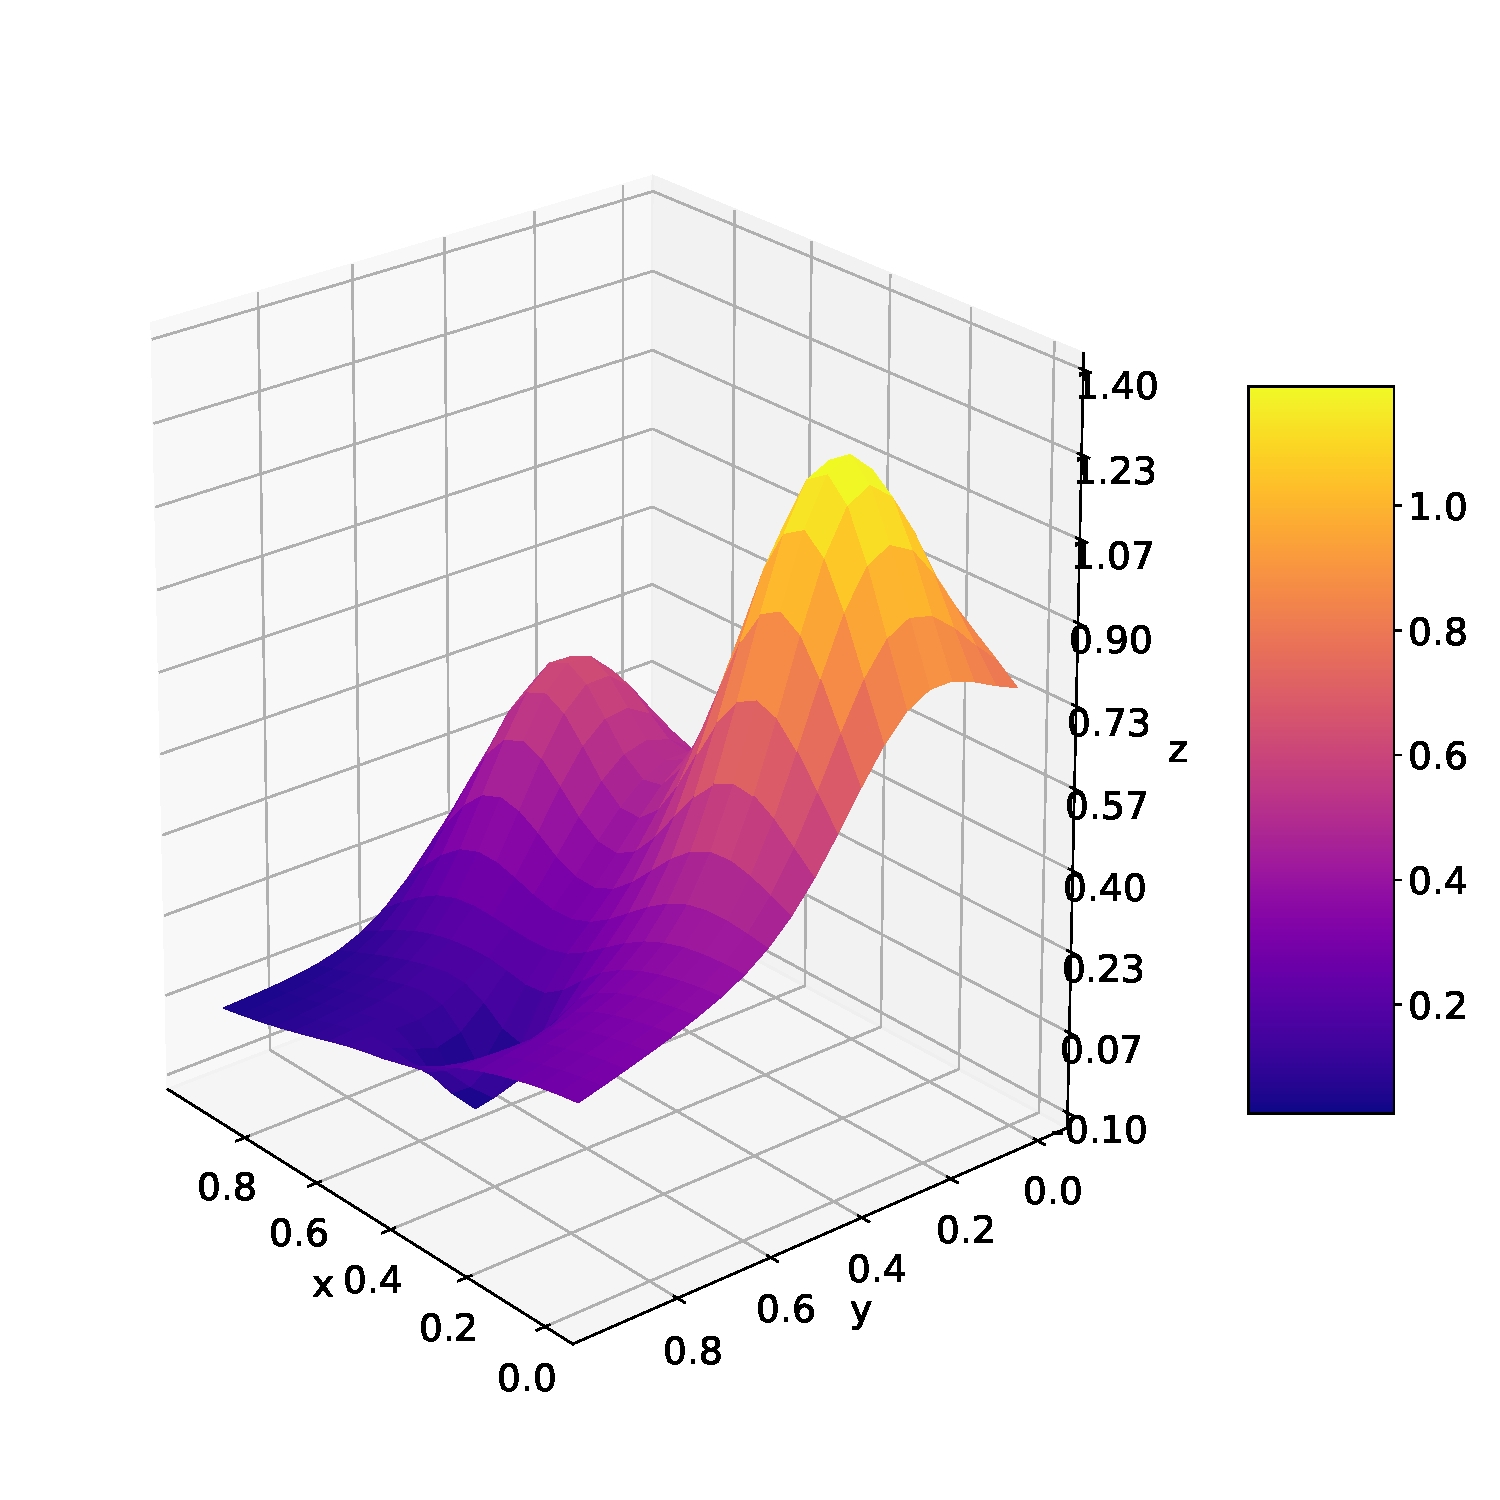
\includegraphics[width=\linewidth]{figures/frankefunc.pdf}
	\captionof{figure}{Illustration of the Franke function.}
	\label{fig:franke3d}
	\end{center}
}

To fit the data from the Franke function we use a two-variable polynomial with the form $[x, y, xy, x^2, y^2,...]$ from which we create the design matrix. 

In our \texttt{Python} code we implement the Franke function, and we construct a function that creates design matrices. The code can be found and seen as a Jupyter Notebook in our GitHub repository (Link found in Appendix \ref{sec:codeappendix}). After we generate the data and design matrix, we split the data into a training set and a test set. The training set is the one used for training our model. Furthermore we implement the Ordinary Least Square and Ridge regression methods using \texttt{NumPy} matrix inversion to find the optimal parameters $\boldsymbol{\beta}^{\mathrm{OLS}}$ and $\boldsymbol{\beta}^{\mathrm{Ridge}}$ from Equations \ref{eq:beta-ols} and \ref{eq:ridge-beta}. Then we implement the LASSO regression from \texttt{Scikit-Learn} and use the built in functionality to find $\boldsymbol{\beta}^{\mathrm{LASSO}}$. With these models we add two different resampling techniques; bootstrap and $K$-fold cross validation. Using all this we assess the models, study the MSE and bias-variance trade-off to find out which of our models perform best, and at what complexity (polynomial degree) and $\lambda$ (if Ridge or LASSO regression) they provide the best results.


Subsequently the same methods were applied to a real dataset using terrain data from the region near Stavanger, Norway, retrieved from \cite{terrain}. This terrain data is shown in Figure \ref{fig:terrain_data}. 

\multicolfloat{	
    \begin{center}
	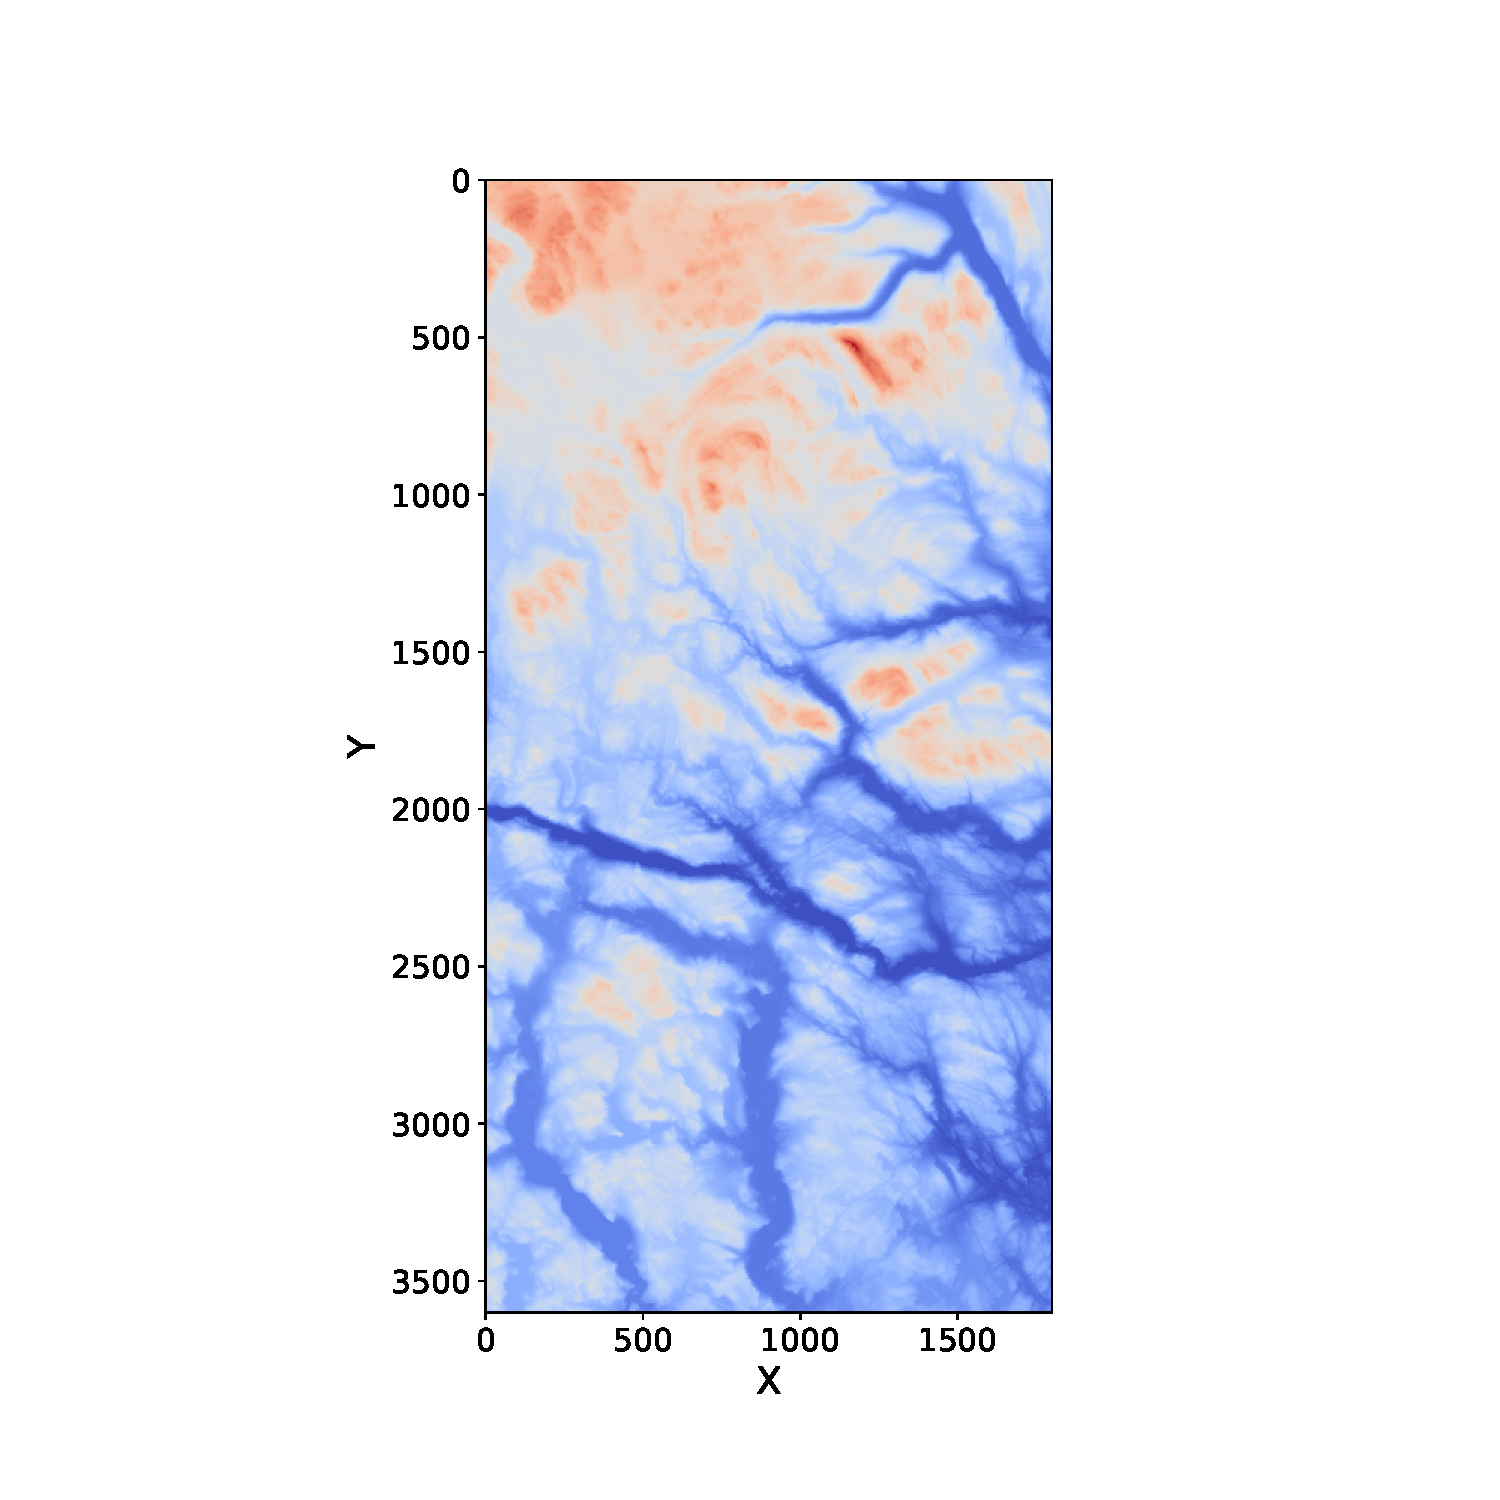
\includegraphics[width=\linewidth]{figures/terrain_image.pdf}
	\captionof{figure}{The terrain data, taken from a region just outside of Stavanger, Norway.}
	\label{fig:terrain_data}
	\end{center}
}

We apply the same regression models as we did on the Franke function, and used $K$-fold cross validation for resampling. To do this we slice the real data up, so that we just use a set amount of data points to train the algorithms on. This also gives us the opportunity to study how well our models can reproduce the terrain.


Implementing the regression methods proved to be fairly trivial, as Ordinary Least Squares and Ridge regression merely entailed matrix inversion problems solvable by \texttt{NumPy} modules. For LASSO we used \texttt{Scikit-Learn}, so none of these regression methods required implementing complex algorithms. For the $K$-fold cross validation we however had to build an algorithm (see below). The performance of our algorithm were compared with the one from \texttt{Scikit-Learn}, showing similar MSE scores (see Fig. \ref{fig:MSE_kfold_franke}).

\begin{algorithm}[H]
\SetAlgoLined
\KwResult{MSE values for each polynomial degree}
 \For{Each polynomial degree }{
  Split data in K-equal parts\;
  \For{Each of the parts}{
   Use selected part for training, and the rest for test\;
   Perform linear regression and return the MSE\;
   }{
   The return the mean of the K different MSE values.\;
  }
 }
 \caption{$K$-fold Cross Validation}
\end{algorithm}


Many of the methods rely on randomly shuffling and/or selecting data. In order to avoid setting a random seed for all the runs, we implemented a repetition loop for the terrain data, where we just looped over the complexities and/or $\lambda$'s. The output MSE was then scored as a mean over all the repetitions. This proved to be rather time consuming.


\section{Results}\label{sec:results}
The results from both the Franke function data and terrain data is presented in this section, and discussed in Section \ref{sec:discussion}. In all the following results we have used scaling of the data. 

\subsection{Franke function analysis}

The first step in the analysis of the data generated using the Franke function was to implement the Ordinary Least Square regression method. The amount of data we generated is specified in the following figures as the $n$ number, which indicates how many data points we used, as in we use $n$ $x$-values and $n$ $y$-values. All the data for the Franke function use a noise factor of $0.1$.

As this was implemented we found the confidence intervals of the parameters $\boldsymbol{\beta}^{\mathrm{OLS}}$ from computing their variances. The result with 95\% confidence intervals is shown in Figure \ref{fig:beta-confidence}. 

\multicolfloat{	
    \begin{center}
	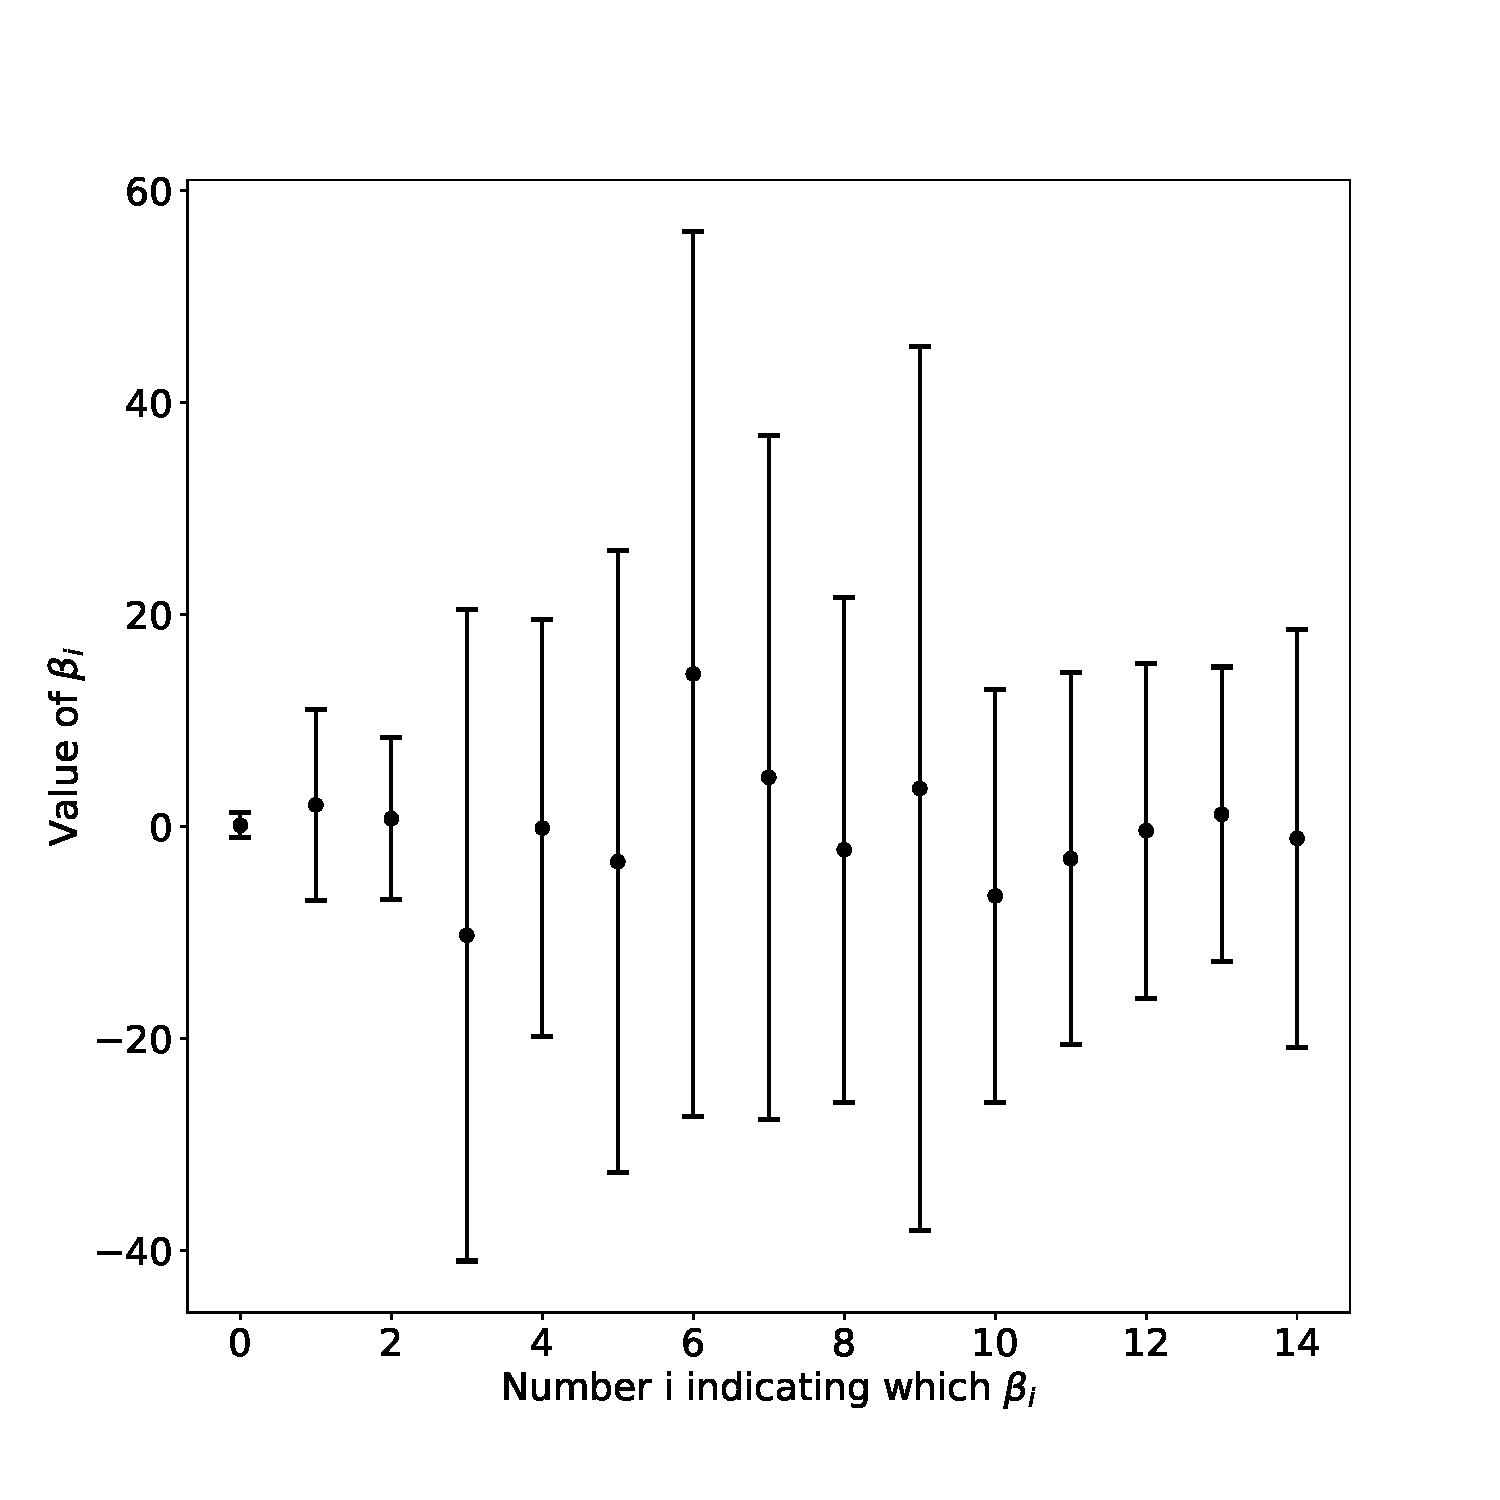
\includegraphics[width=\linewidth]{figures/confidence_intervals_beta.pdf}
	\captionof{figure}{The OLS parameters $\boldsymbol{\beta}^{\mathrm{OLS}}$ for the Franke function, plotted with 95\% confidence intervals. Plotted for a polynomial degree of $4$ and $n = 500$.}
	\label{fig:beta-confidence}
	\end{center}
}

Furthermore we calculated the MSE and $\mathrm{R}^2$ values obtained from the OLS, Ridge and LASSO methods with a complexity of $9$. These results are presented in Table \ref{tab:task1a-values}. Here we only chose one value for the hyperparameter for Ridge and LASSO, namely $\lambda = 0.01$.


\begin{Table}
\captionof{table}{The $\mathrm{R}^2$ score and $\mathrm{MSE}$ for both the training and test data using Ordinary Least Squares, Ridge and LASSO on the Franke function data. The data is scaled. These values were retrieved using a complexity (polynomial degree) of $9$, $n = 1000$ x and y values and a noise factor of $0.1$ in our program. For the Ridge and LASSO we used a hyperparameter $\lambda = 0.01$.}
\centering
\begin{tabular}{p{0.15\linewidth}p{0.15\linewidth}p{0.15\linewidth}p{0.15\linewidth}p{0.15\linewidth}}
\hline
\hline
Method & $\mathrm{R}_{\mathrm{Train}}^2$ & $\mathrm{MSE}_{\mathrm{Train}}$ &   $\mathrm{R}_{\mathrm{Test}}^2$ & $\mathrm{MSE}_{\mathrm{Test}}$ \\
\hline
OLS & $0.8897$ & $0.0096$ & $0.8768$ & $0.0103$  \\
Ridge & $0.8693$ & $0.0113$ & $0.8712$ & $0.0108$  \\
LASSO & $0.6349$ & $0.0318$ & $0.6399$ & $0.0302$  \\
\hline
\hline
\end{tabular}
\label{tab:task1a-values}
\end{Table}

To study the bias-variance trade-off we used the OLS method and implemented the Bootstrap resampling technique. First we analysed how the MSE changed for increasing complexity for both the training and test data, as well as for the test data with Bootstrap. The bias and variance were also plotted for the same complexities and numbers of data points. This is shown in Figure \ref{fig:MSE_bias_var_franke}.


\multicolfloat{	
    \begin{center}
	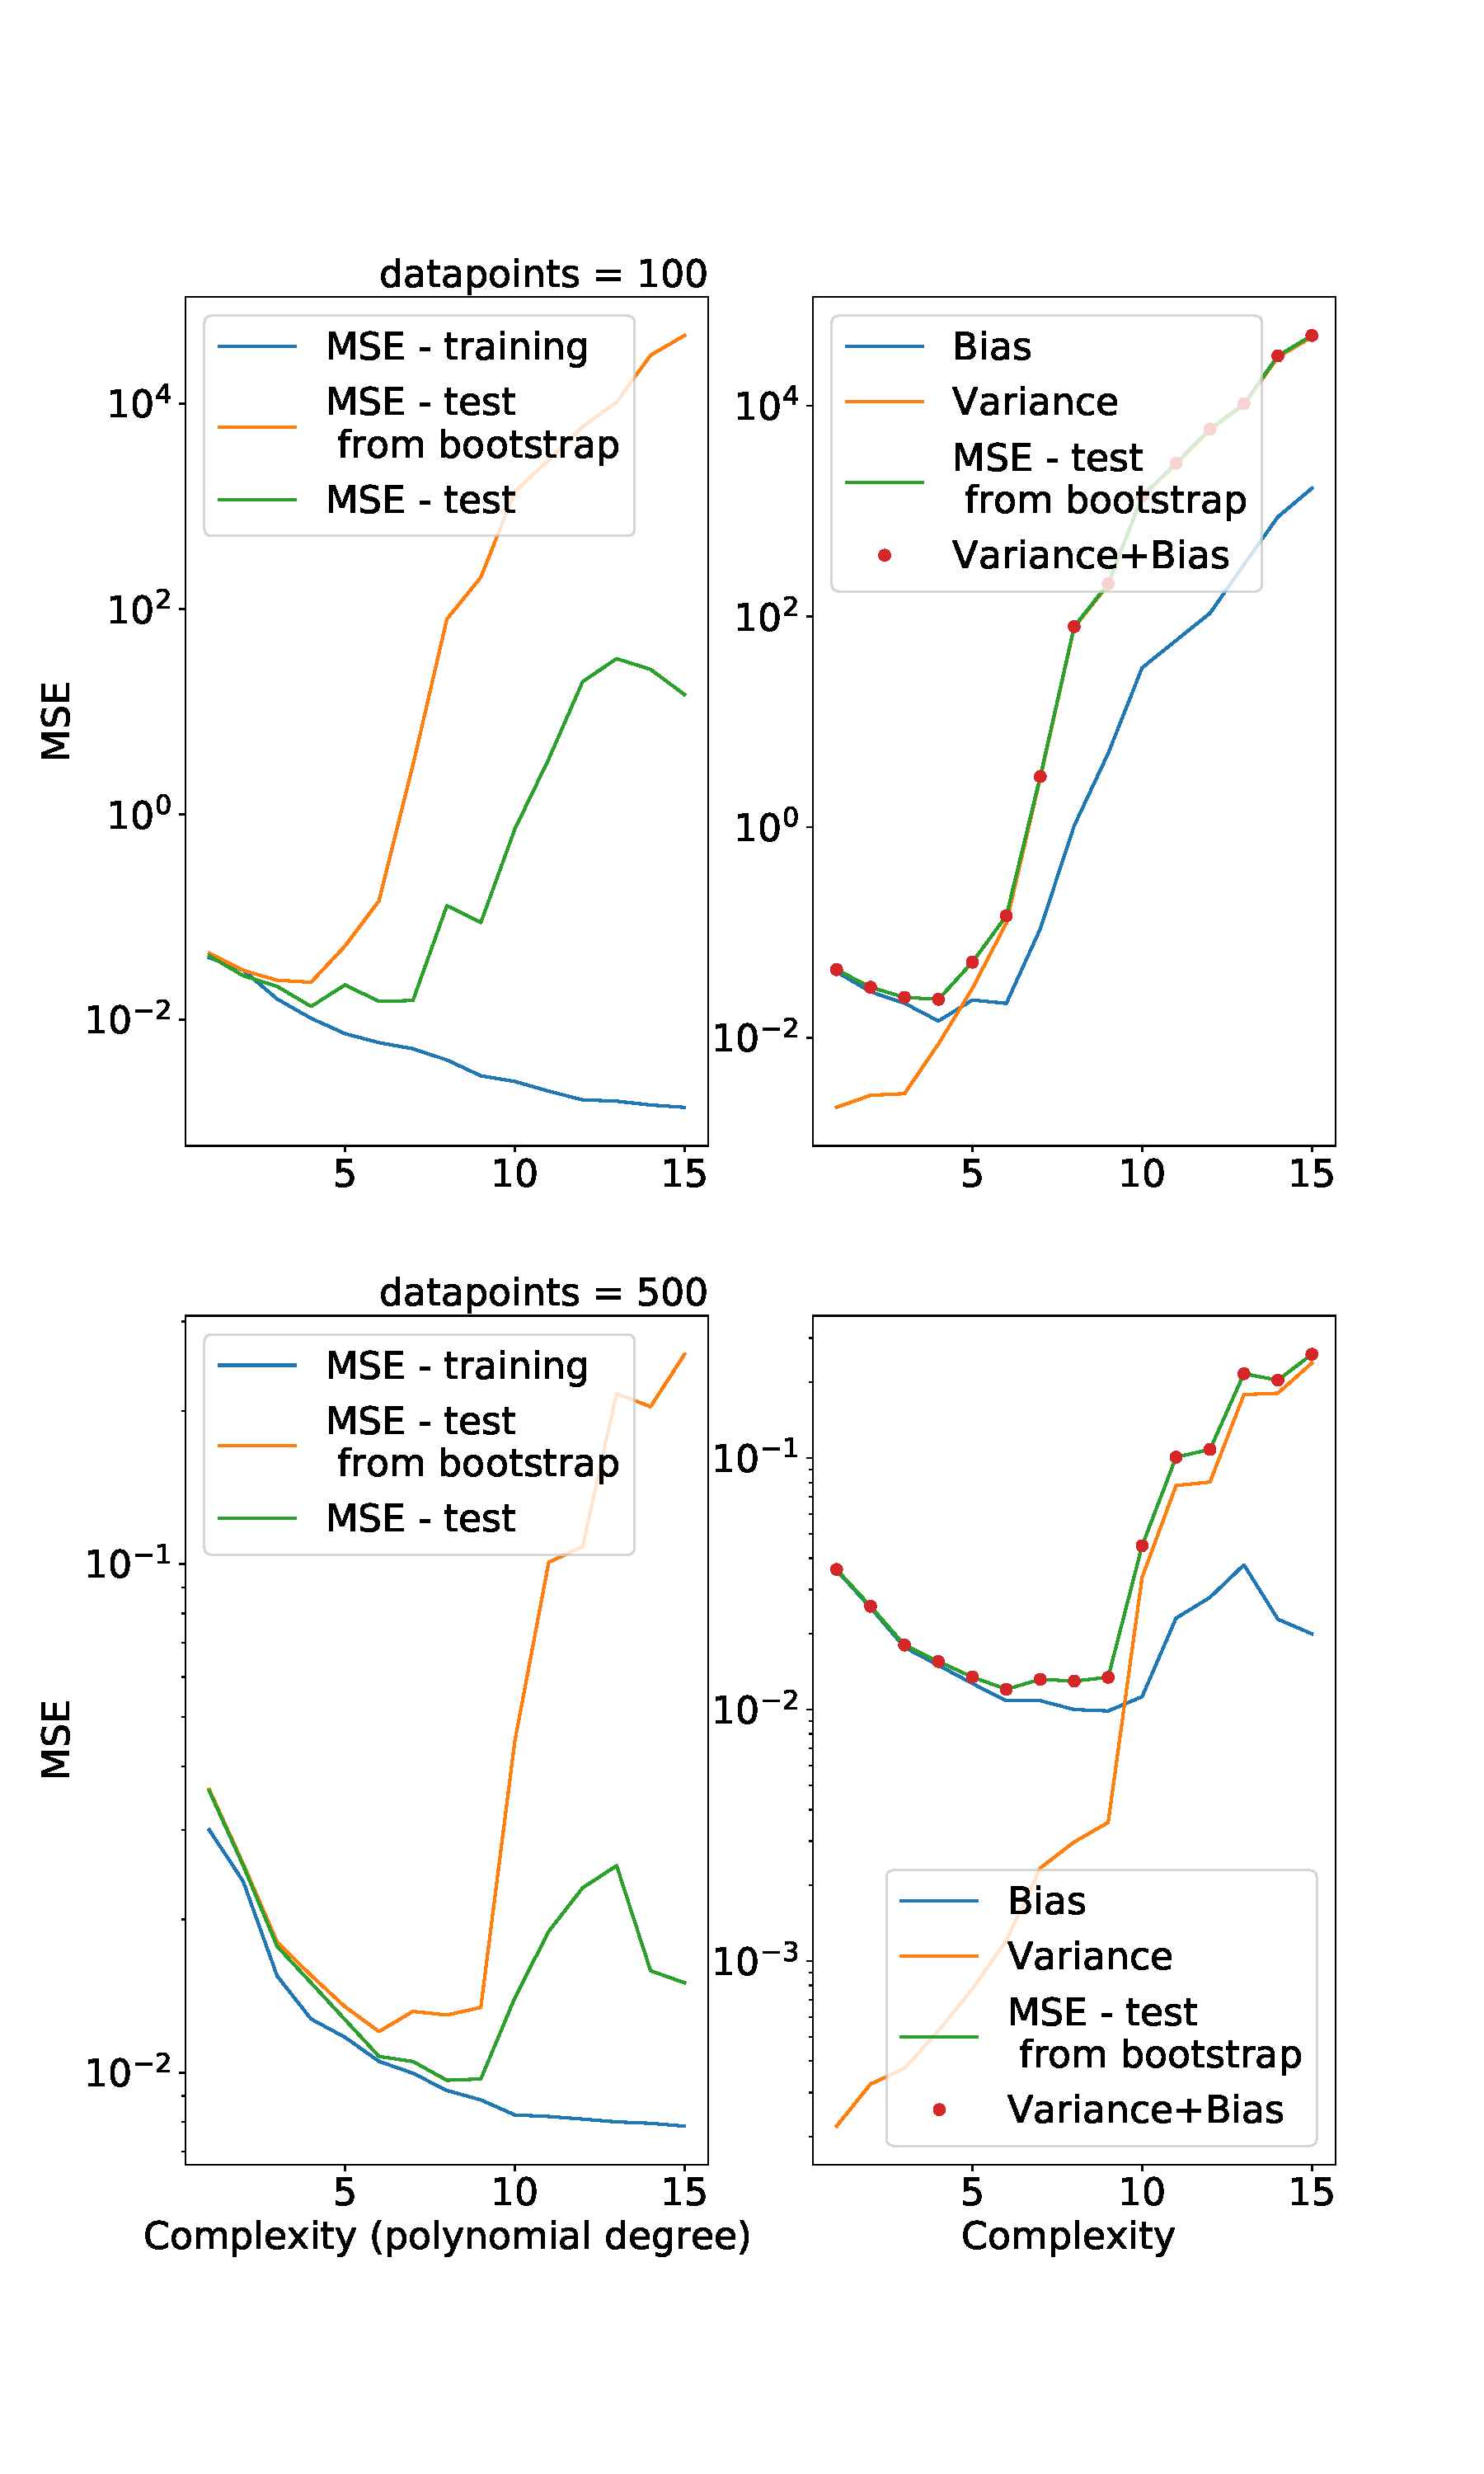
\includegraphics[width=\linewidth]{figures/MSE_bias_variance_franke.pdf}
	\captionof{figure}{The MSE scores (left) for the Franke function data with and without Bootstrap resampling. The ones with Bootstrap resampling was run with $100$ bootstraps. Plots on the right illustrates the bias-variance trade-off. The upper plots are made with $n = 100$ datapoints, while the lower are made with $n = 500$ datapoints.}
	\label{fig:MSE_bias_var_franke}
	\end{center}
}

Additionally we implemented the $K$-fold cross validation resampling technique. We studied how the MSE for the OLS method changed in relation to the complexity, and compared the MSE test of both Bootstrap and cross validation to the MSE of the training data. We studied the effects of additional folds, and looked at cases with 5, 7 and 10 fold cross validation. To study how our $K$-fold cross validation algorithm performed we included the results from the \texttt{Scikit-Learn} cross validation method. The results are presented in Figure \ref{fig:MSE_kfold_franke}.

\multicolfloat{	
    \begin{center}
	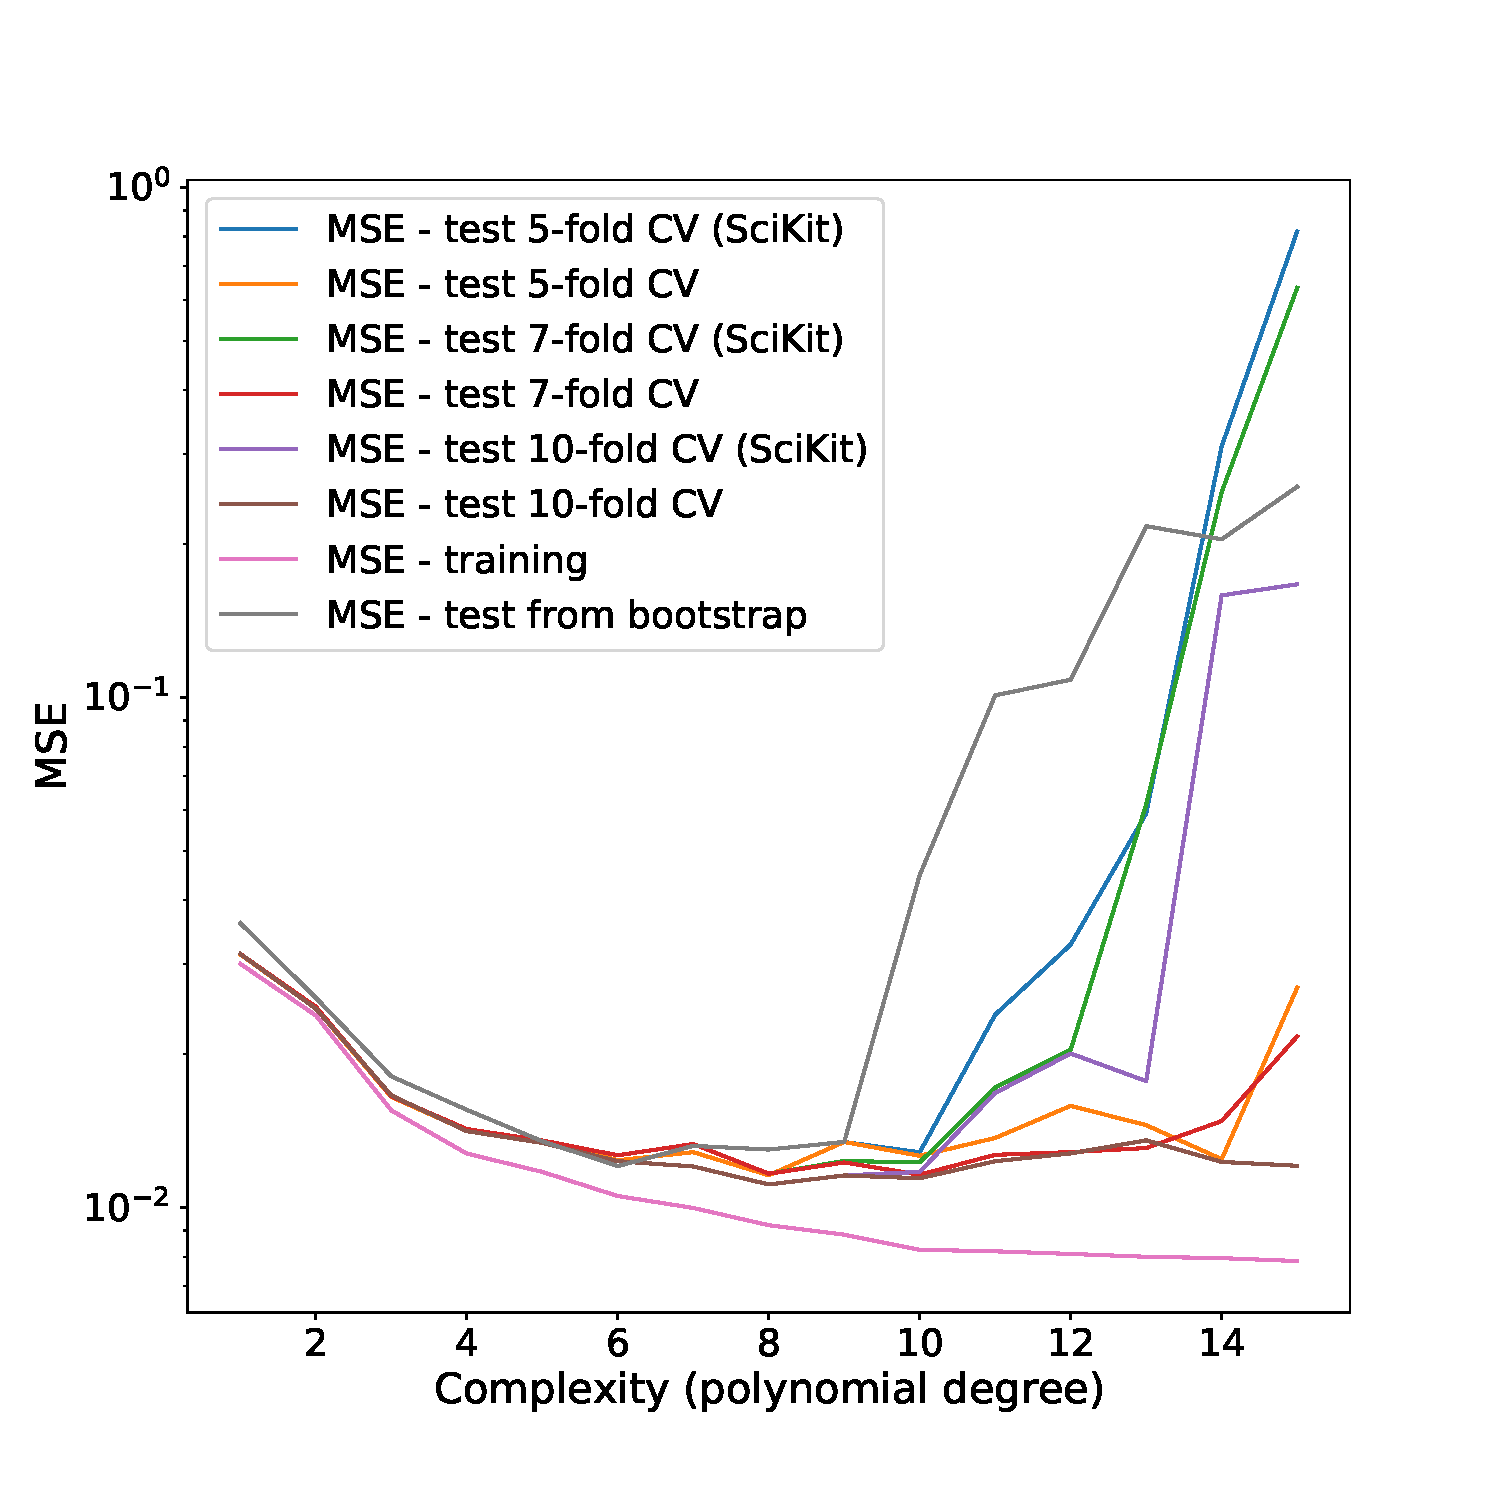
\includegraphics[width=\linewidth]{figures/mse_kfold_bootstrap_franke_500_points.pdf}
	\captionof{figure}{The MSE for the OLS method with $K$-fold cross-validation and with bootstrap resampling on the data from the Franke function, with $n = 500$. Different values of $K$-folds are shown, and compared with the \texttt{Scikit-Learn} $K$-fold method.}
	\label{fig:MSE_kfold_franke}
	\end{center}
}


Ridge regression was subsequently implemented and the MSE with and without resampling methods were plotted versus the values of the hyperparameter $\lambda$, as shown in Figure \ref{fig:MSE_ridge_franke}. The bias and variance for the Ridge regression with Bootstrap was also plotted versus $\lambda$ for a complexity of $10$, as shown in Figure \ref{fig:biasvariance_ridge_franke}.

Likewise the MSE was studied in relation to the hyperparameter $\lambda$ for the LASSO regression as well. The results can be seen in Figure \ref{fig:MSE_LASSO_franke}. The bias and variance was also plotted for LASSO with Bootstrap at a complexity of $10$, shown in Figure \ref{fig:biasvariance_LASSO_franke}. 


\multicolfloat{	
    \begin{center}
	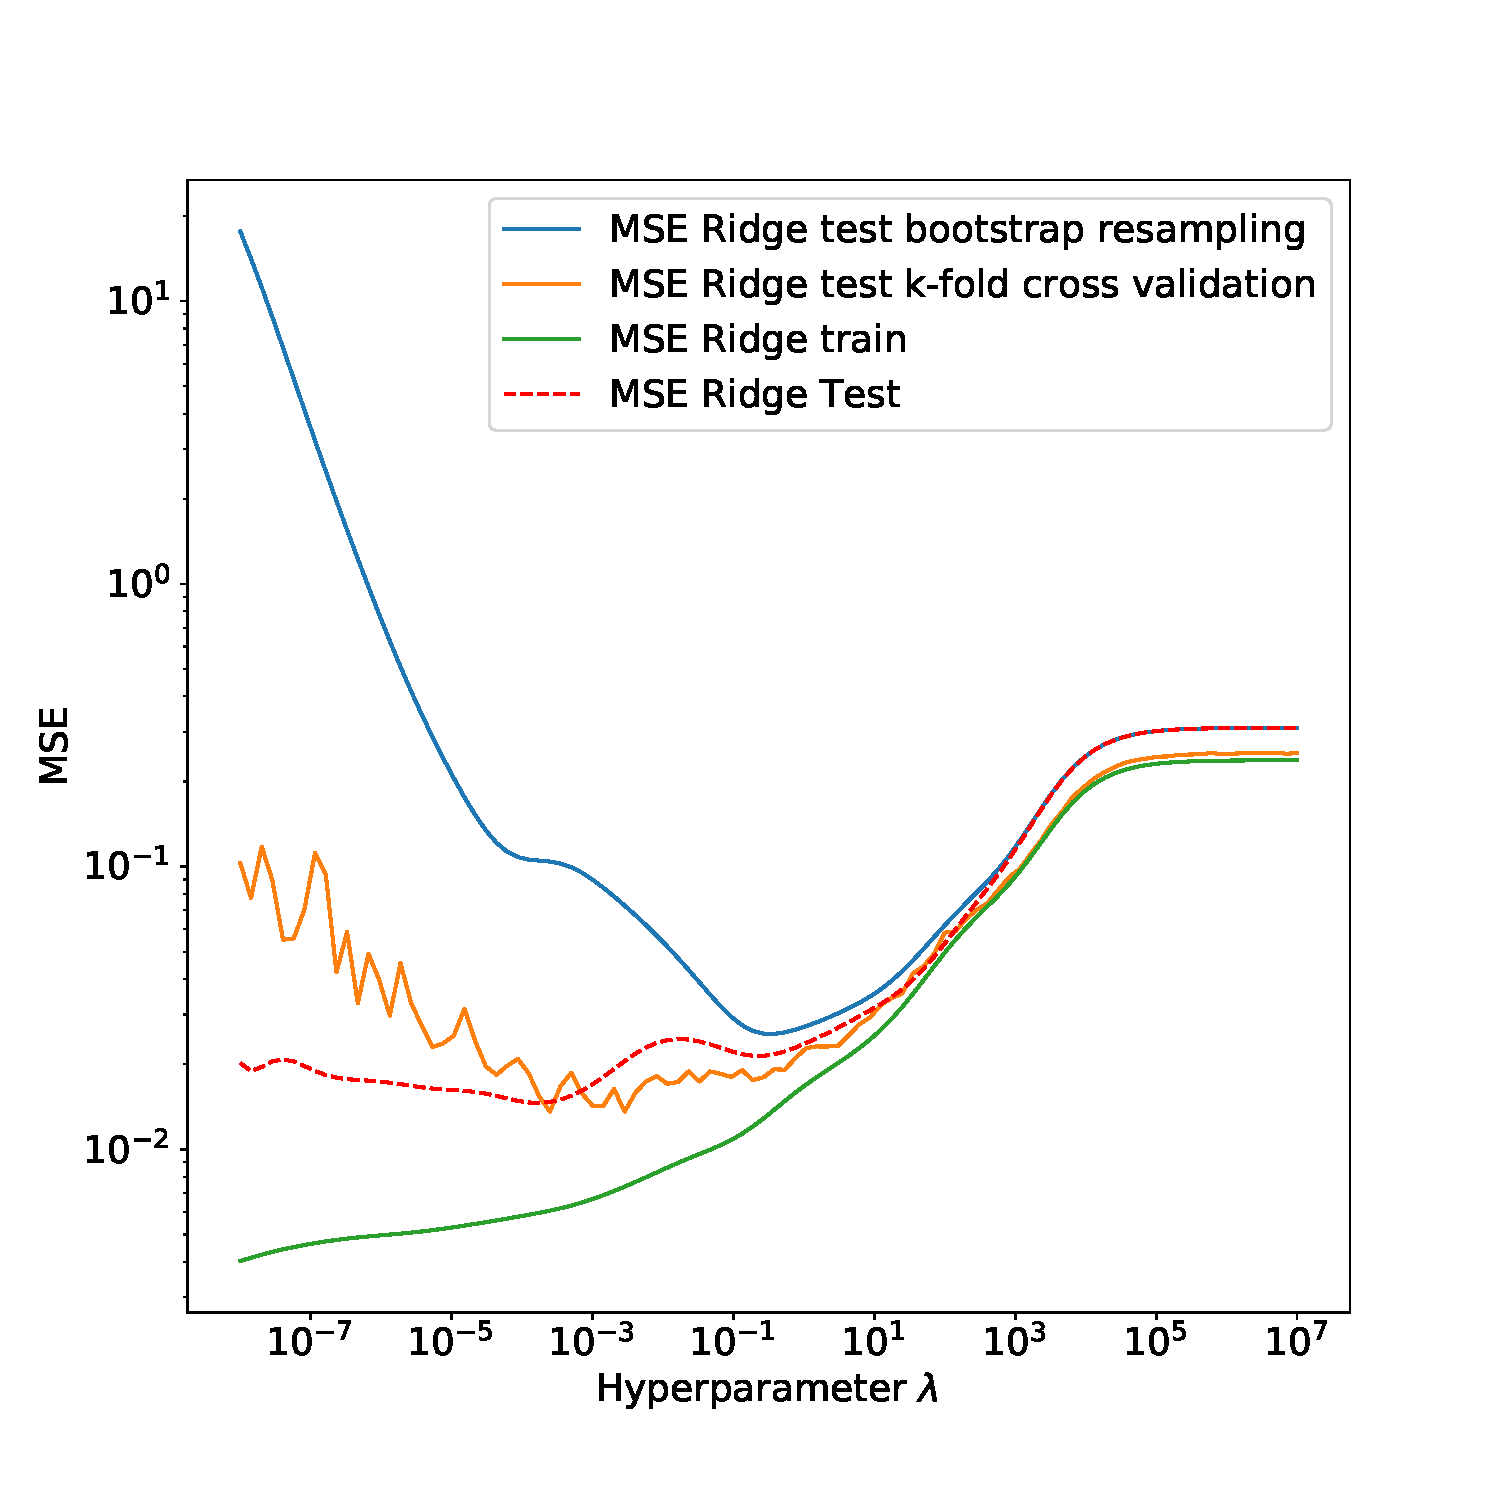
\includegraphics[width=\linewidth]{figures/MSE_ridge_franke.pdf}
	\captionof{figure}{The MSE for the Franke function data, fitted with the Ridge regression method for a complexity of $10$ and $n = 100$ with $100$ $\lambda$ values from $10^{-8}$ to $10^{7}$. Resampling with the Bootstrap method with $100$ bootstraps, and cross validation with the $K$-fold method for $K = 7$ folds are also applied to the Ridge regression and shown here.}
	\label{fig:MSE_ridge_franke}
	\end{center}
}

\multicolfloat{	
    \begin{center}
	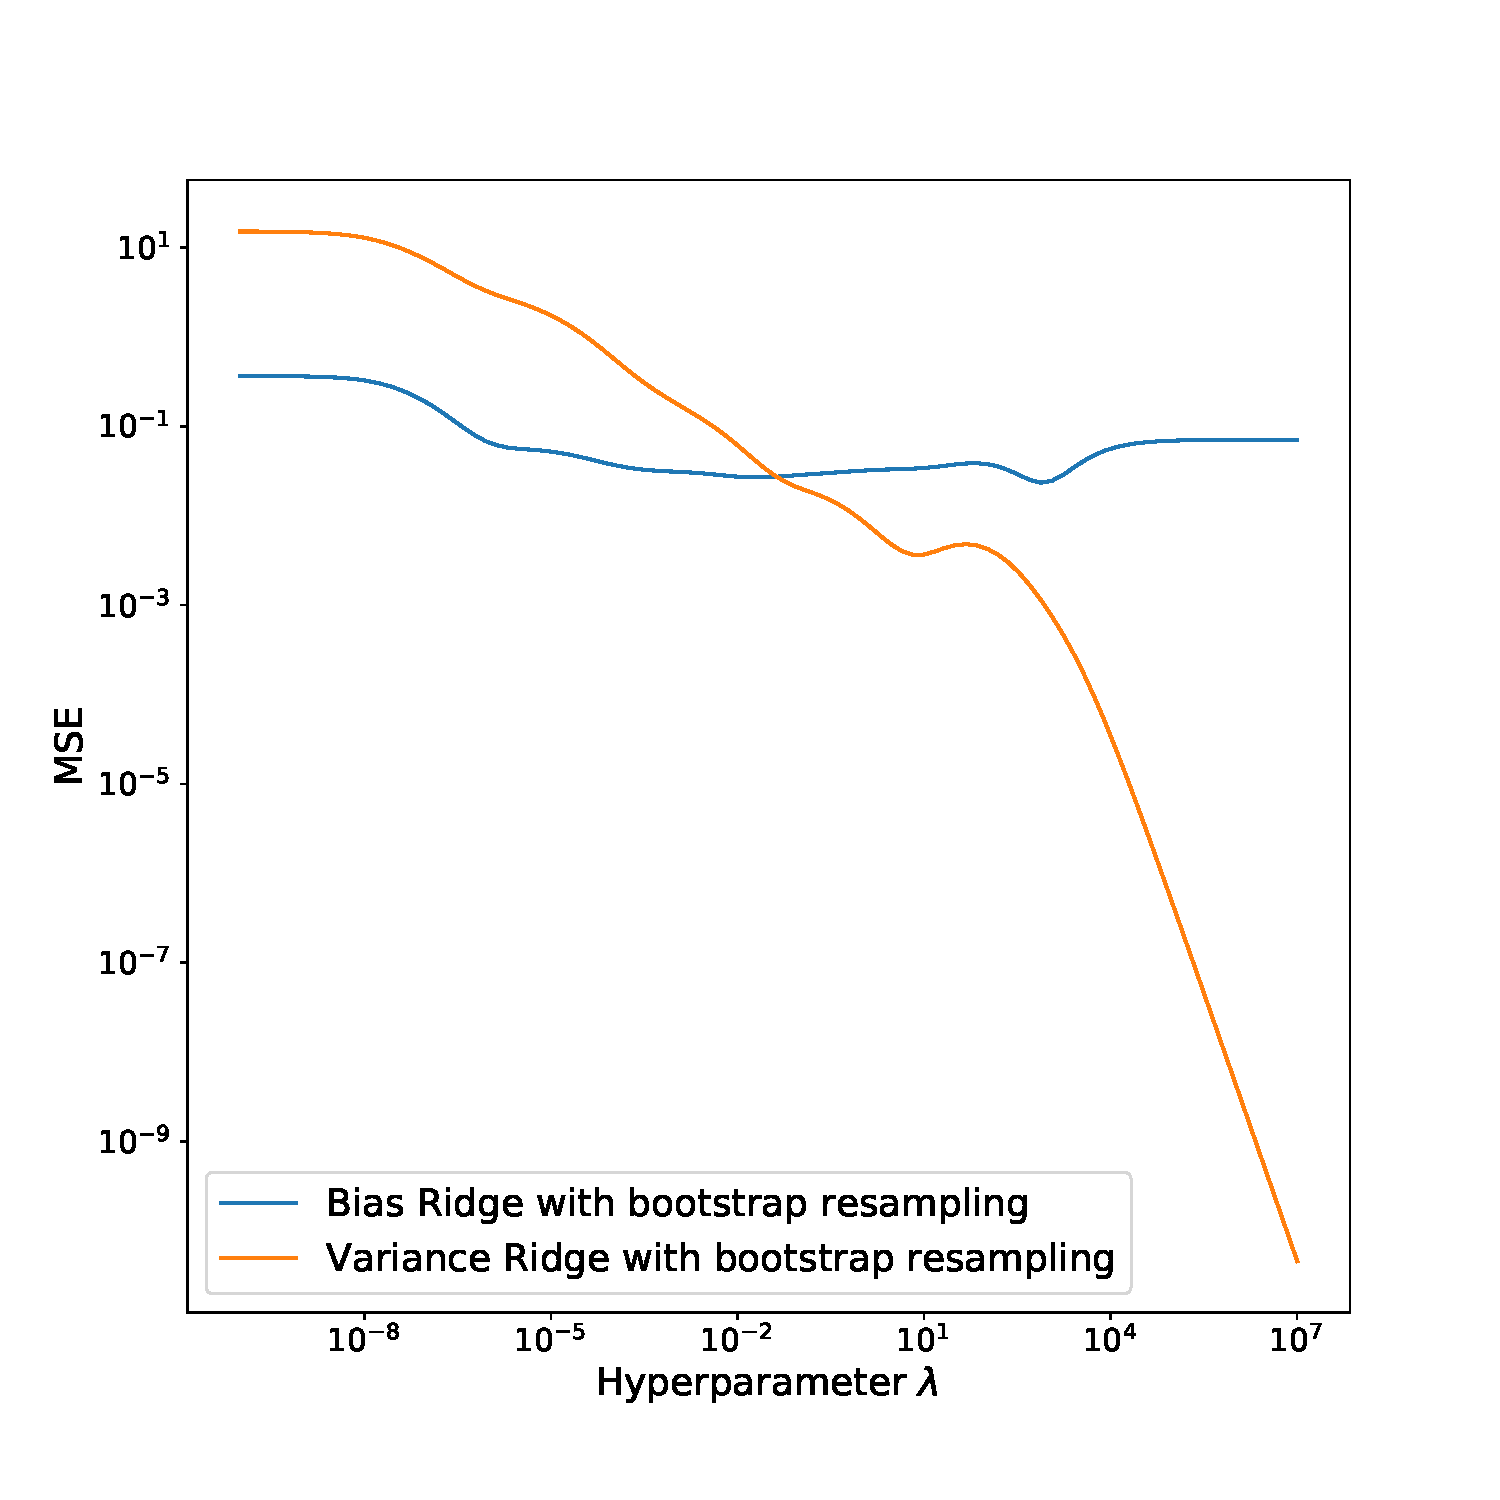
\includegraphics[width=\linewidth]{figures/biasvariance_ridge_franke.pdf}
	\captionof{figure}{Bias-variance trade-off for the Franke function data, fitted with the Ridge regression method with the same complexity, datapoints, $\lambda$ and bootstraps as in Figure \ref{fig:MSE_ridge_franke}.}
	\label{fig:biasvariance_ridge_franke}
	\end{center}
}



\multicolfloat{	
    \begin{center}
	\includegraphics[width=\linewidth]{figures/MSE_LASSO_franke.pdf}
	\captionof{figure}{The MSE for the Franke function data, fitted with the LASSO regression method for a complexity of $10$, $n = 100$ and $100$ $\lambda$ values from $10^{-5}$ to $10^0$. Resampling with the Bootstrap method using $100$ bootstraps, and cross validation with the $K$-fold method for $k = 7$ folds are also applied to the LASSO regression and shown here.}
	\label{fig:MSE_LASSO_franke}
	\end{center}
}

\multicolfloat{	
    \begin{center}
	\includegraphics[width=\linewidth]{figures/biasvariance_LASSO_franke.pdf}
	\captionof{figure}{Bias-variance trade-off for the Franke function data, fitted with the LASSO regression method for the same complexity, datapoints, $\lambda$ and bootstraps as in Figure \ref{fig:MSE_LASSO_franke}. Not plotted with logarithmic y-axis to show the variance.}
	\label{fig:biasvariance_LASSO_franke}
	\end{center}
}


\subsection{Terrain data}
For the real terrain data we performed our analysis using OLS, Ridge and LASSO both with and without $K$-fold cross validation as resampling. Throughout our terrain analysis we read the complete terrain data, and then slice it up so that we get fewer datapoints to evaluate our models against the real terrain data. In all the analysis below we have used $144$ $x$ and $y$ values, and $144$ terrain data values. For the K-fold cross validation we here used $7$ folds for all plots except Figure \ref{fig:MSE_ols_kfold_terrain}.

The MSE found for OLS is shown in Figure \ref{fig:MSE_ols_kfold_terrain}. 

\multicolfloat{	
    \begin{center}
	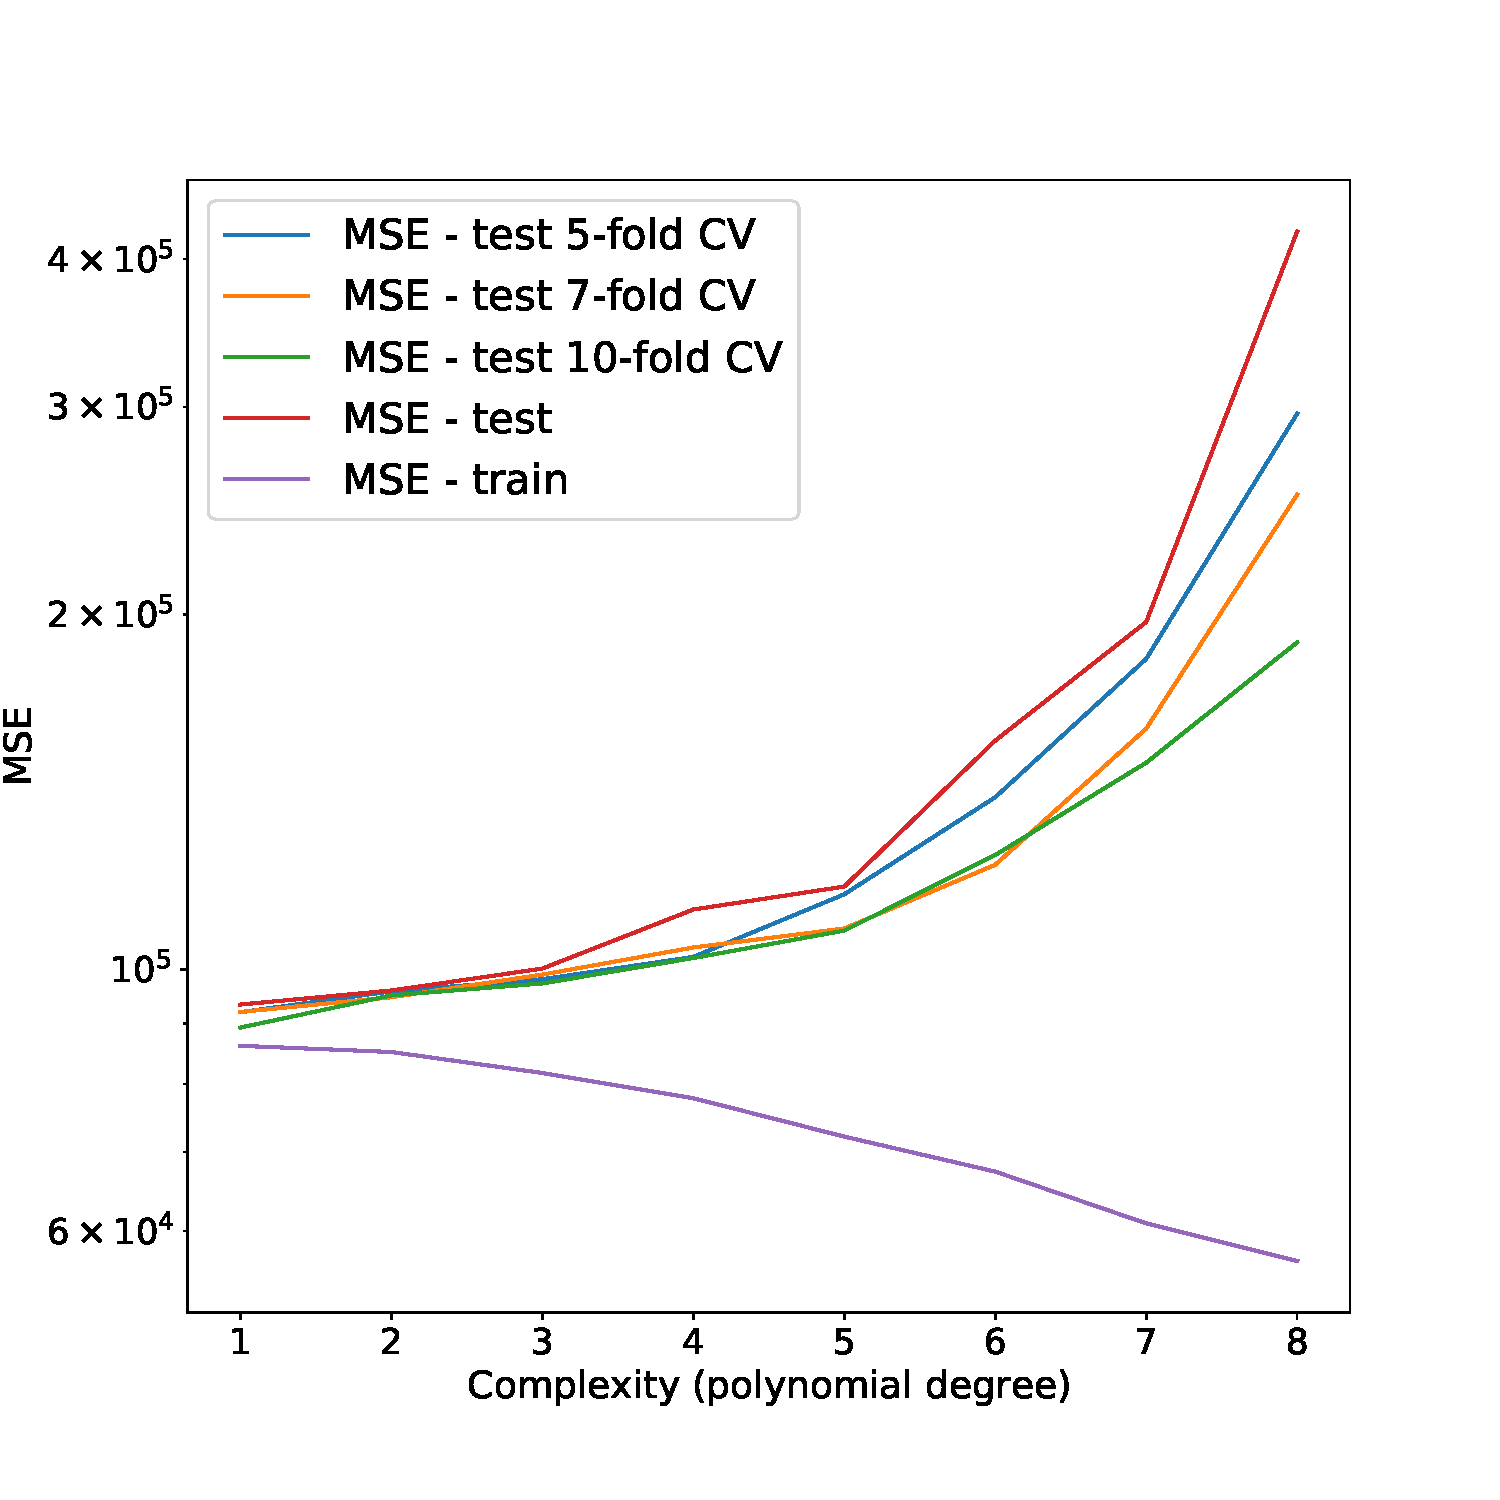
\includegraphics[width=\linewidth]{figures/mse_kfold_terrain.pdf}
	\captionof{figure}{The MSE of our OLS fit on the Terrain, here shown with different $K$-fold values.}
	\label{fig:MSE_ols_kfold_terrain}
	\end{center}
}

For the Ridge regression we plotted the MSE compared to the hyperparameter $\lambda$, for two different complexities, namely $10$ and $20$. The results are shown in Figures \ref{fig:MSE_ridge_terain_poly10} and \ref{fig:MSE_ridge_terain_poly20}. 

\multicolfloat{	
    \begin{center}
	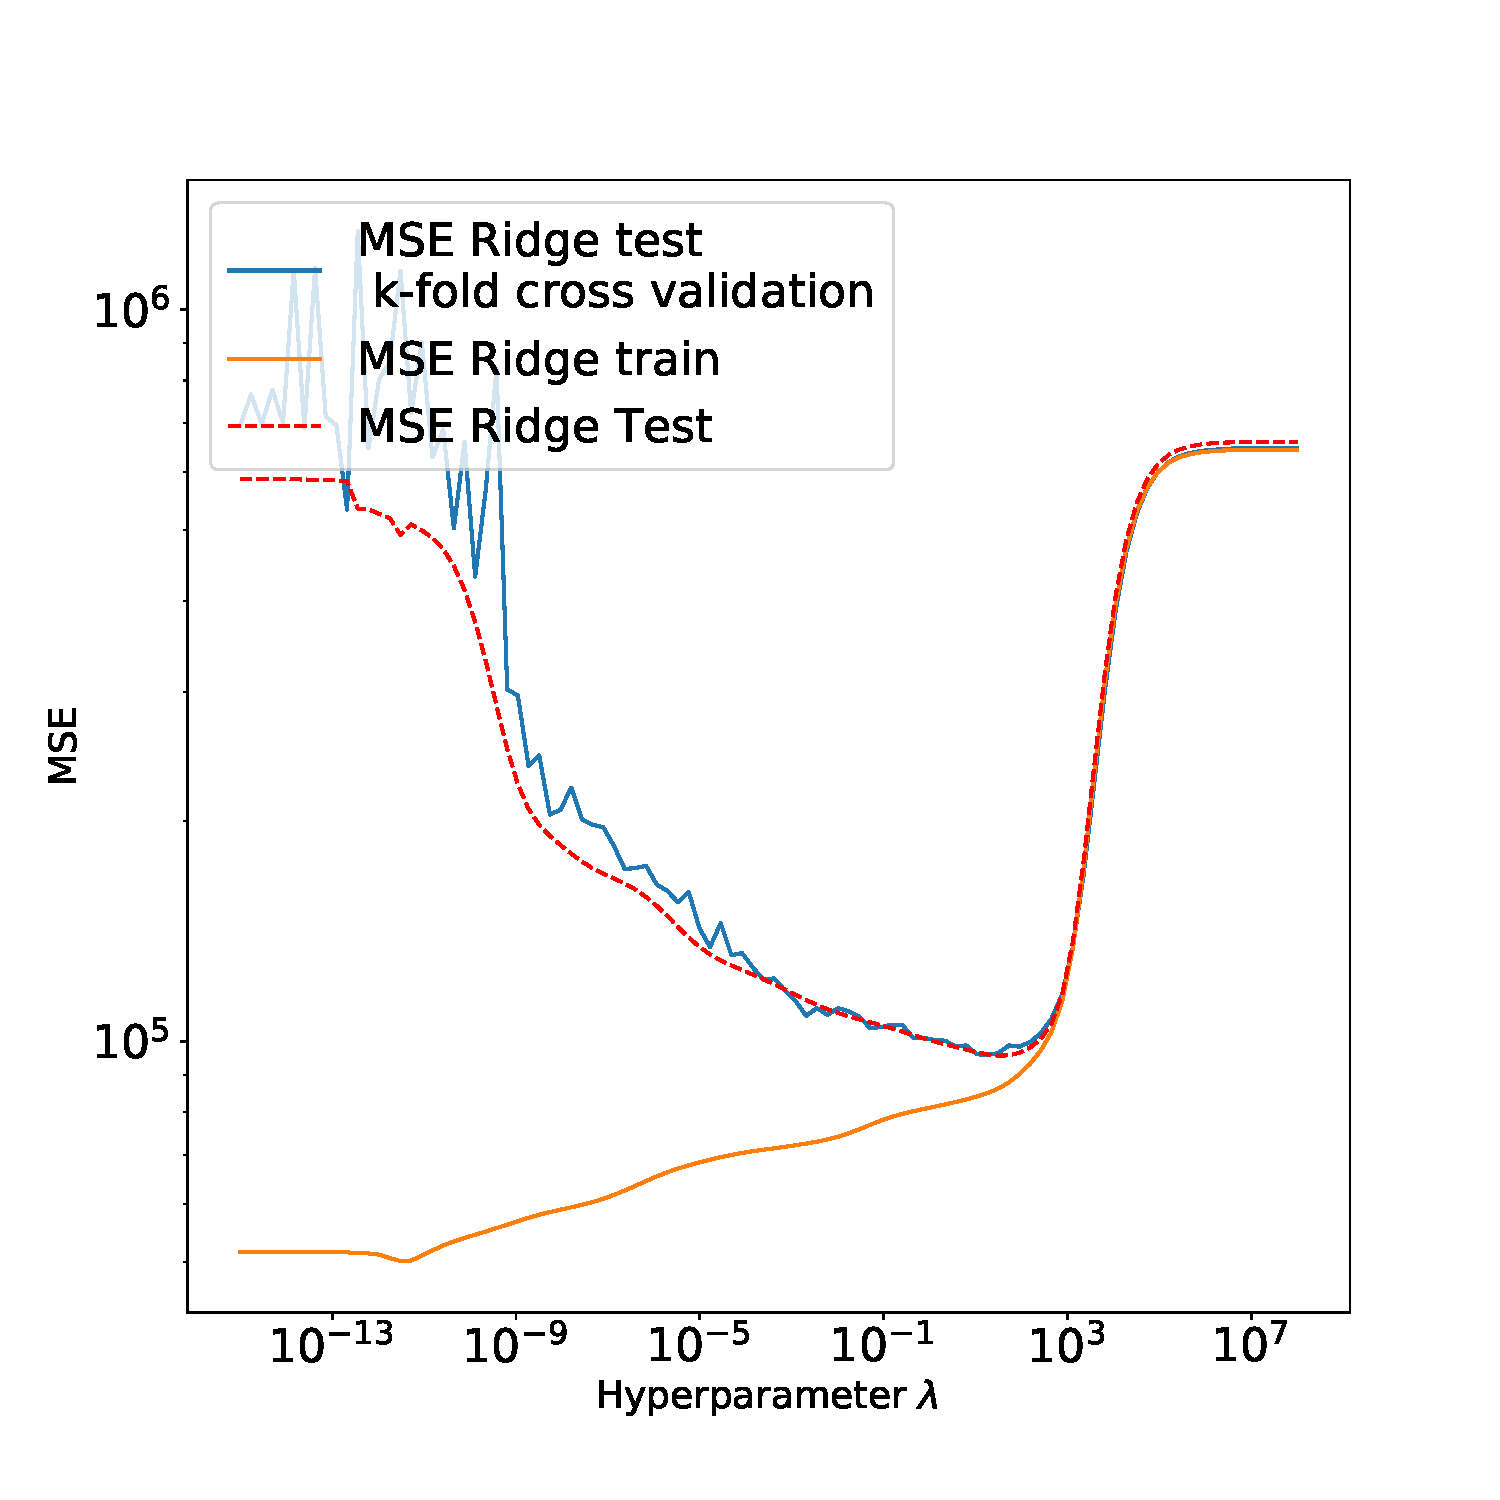
\includegraphics[width=\linewidth]{figures/MSE_ridge_terrain_poly10.pdf}
	\captionof{figure}{MSE for Ridge regression used to fit the terrain data, with $K$-fold cross validation and a polynomial degree of 10.}
	\label{fig:MSE_ridge_terain_poly10}
	\end{center}
}

\multicolfloat{	
    \begin{center}
	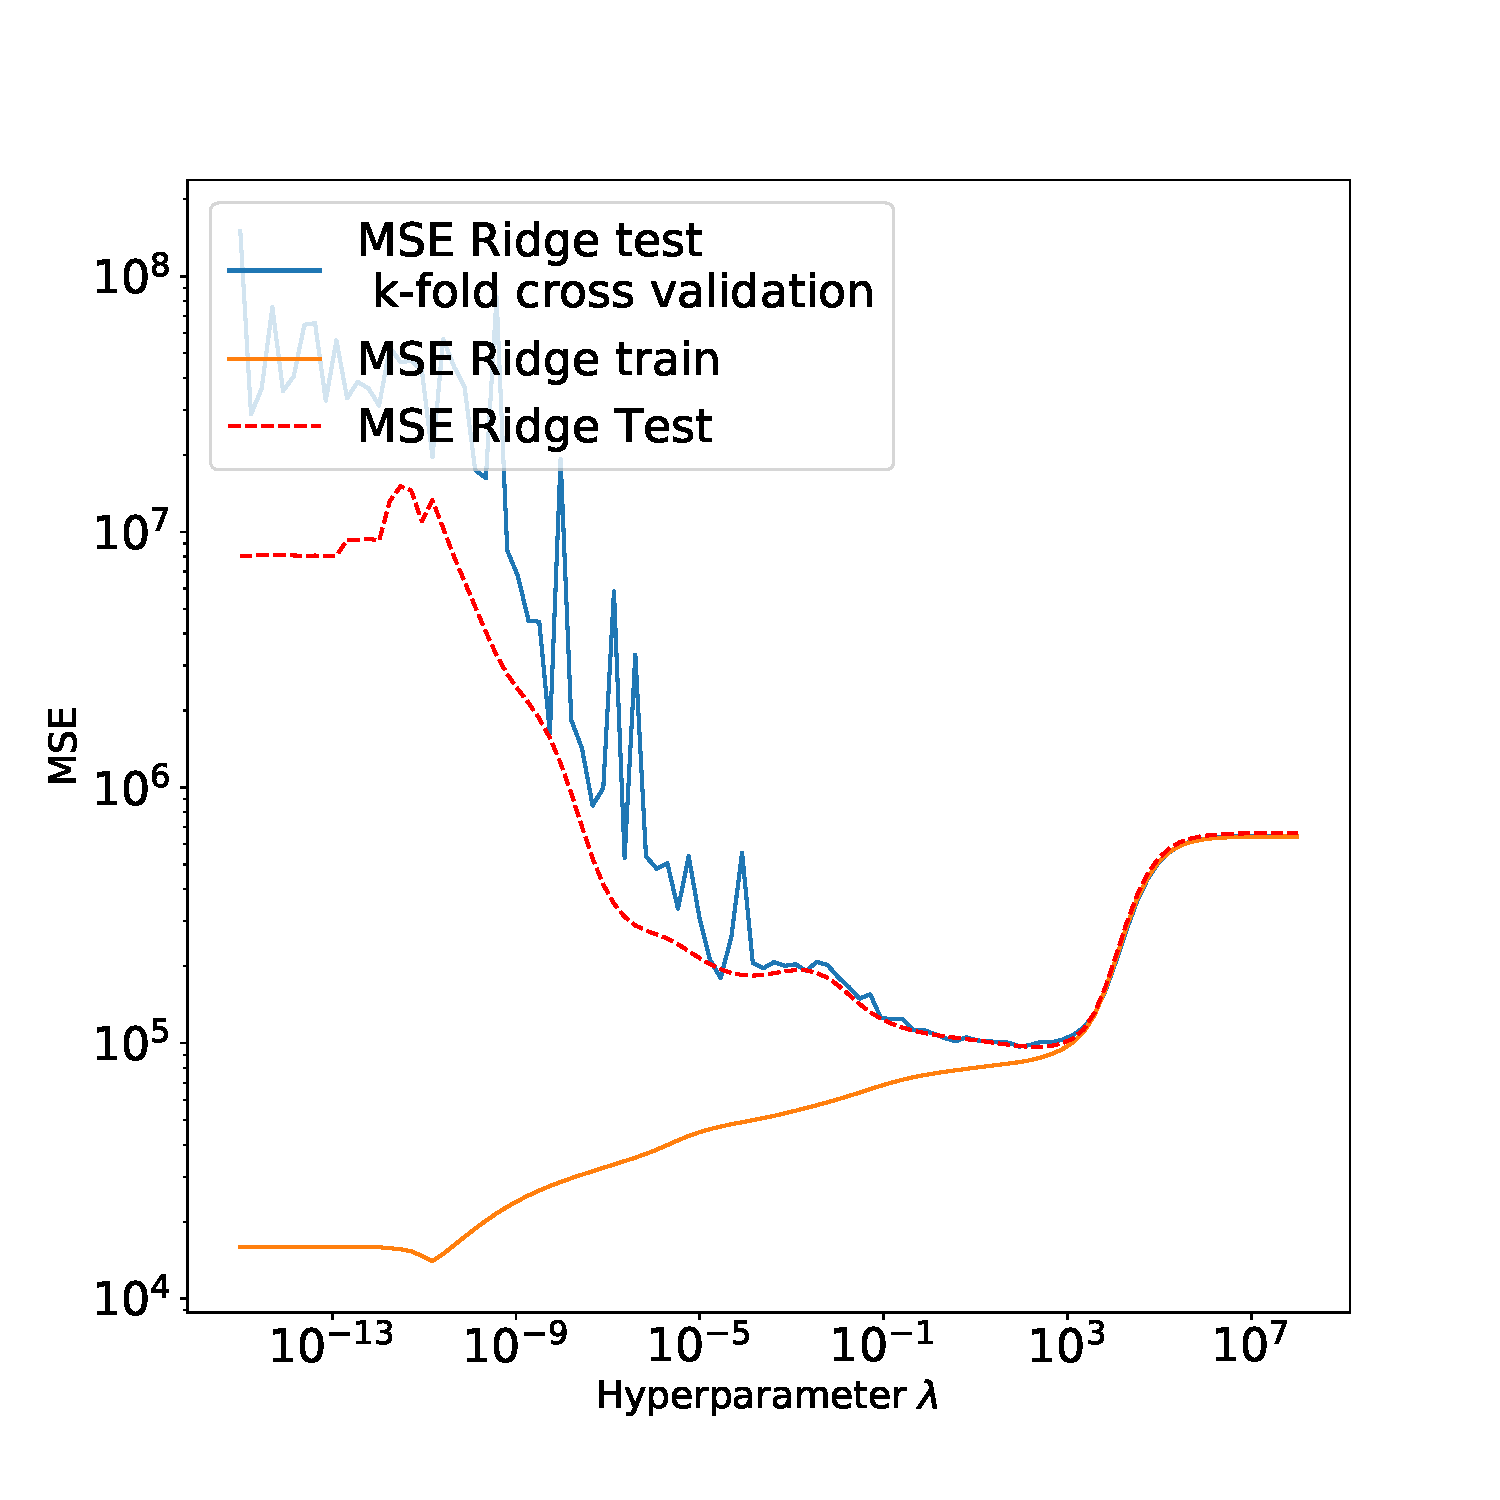
\includegraphics[width=\linewidth]{figures/MSE_ridge_terrain_poly20.pdf}
	\captionof{figure}{MSE for Ridge regression used to fit the terrain data, with $K$-fold cross validation and a polynomial degree of 20.}
	\label{fig:MSE_ridge_terain_poly20}
	\end{center}
}

Similarly, we also compared the MSE for LASSO using the same complexities, $10$ and $20$ to see how it changes with both complexity and $\lambda$. The results are shown in Figures \ref{fig:MSE_LASSO_terain_poly10} and \ref{fig:MSE_LASSO_terain_poly20}.

\multicolfloat{	
    \begin{center}
	\includegraphics[width=\linewidth]{figures/MSE_LASSO_terrain_poly10.pdf}
	\captionof{figure}{MSE for LASSO regression used to fit the terrain data, with $K$-fold cross validation and a polynomial degree of 10.}
	\label{fig:MSE_LASSO_terain_poly10}
	\end{center}
}


\multicolfloat{	
    \begin{center}
	\includegraphics[width=\linewidth]{figures/MSE_LASSO_terrain_poly20.pdf}
	\captionof{figure}{MSE for LASSO regression used to fit the terrain data, with $K$-fold cross validation and a polynomial degree of 20.}
	\label{fig:MSE_LASSO_terain_poly20}
	\end{center}
}

To find the case where Ridge and LASSO regression had the lowest MSE we varied both $\lambda$ and complexity to find the optimal values. These were found in Figures \ref{fig:MSE_optimal_ridge} and \ref{fig:MSE_optimal_LASSO}. Finally we also found the MSE of the OLS fit for the terrain data, and compared this to the Ridge and LASSO method, as shown in Figure \ref{fig:MSE_optimal_ols}.

\multicolfloat{	
    \begin{center}
	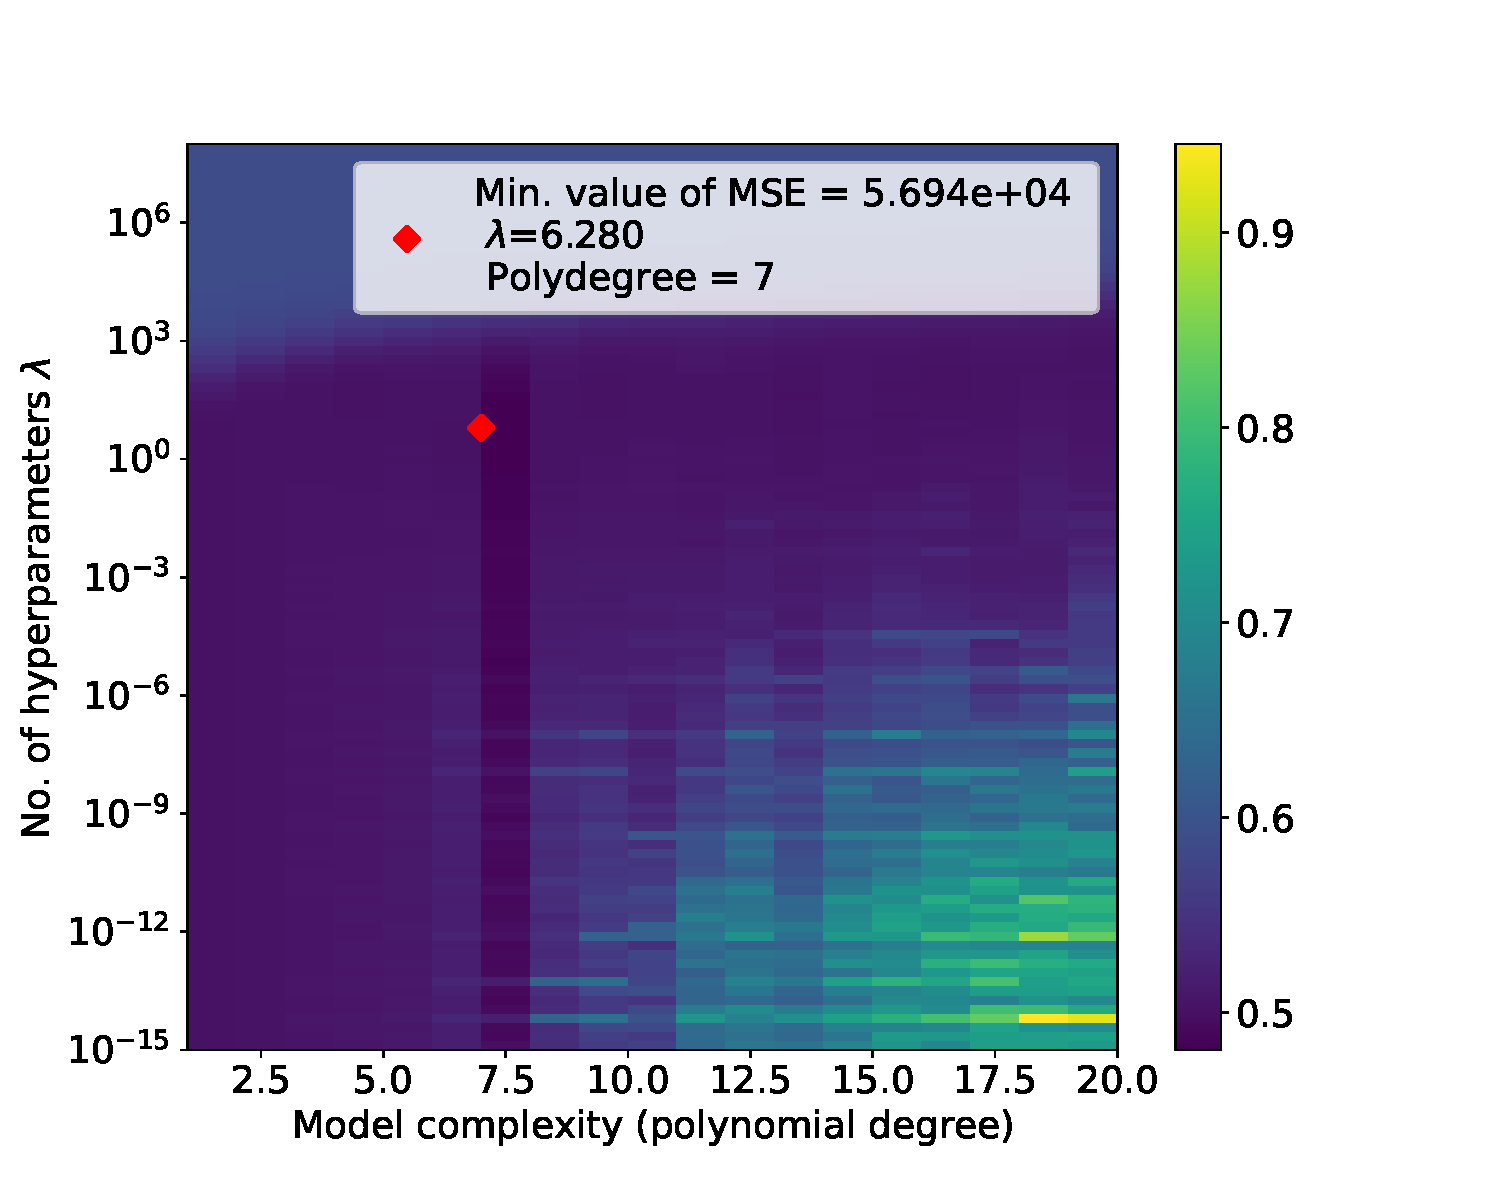
\includegraphics[width=\linewidth]{figures/optimal_mse_ridge.pdf}
	\captionof{figure}{The MSE of our fit on the terrain-data with Ridge regression is plotted against different values of polynomial degree and the hyperparameter $\lambda$. The optimal MSE value we found is marked with the red square.}
	\label{fig:MSE_optimal_ridge}
	\end{center}
}


\multicolfloat{	
    \begin{center}
	\includegraphics[width=\linewidth]{figures/optimal_mse_LASSO.pdf}
	\captionof{figure}{The MSE of our fit on the terrain-data with LASSO regression is plotted against different values of polynomial degree and the hyperparameter $\lambda$. The optimal MSE value we found is marked with the red square.}
	\label{fig:MSE_optimal_LASSO}
	\end{center}
}


\multicolfloat{	
    \begin{center}
	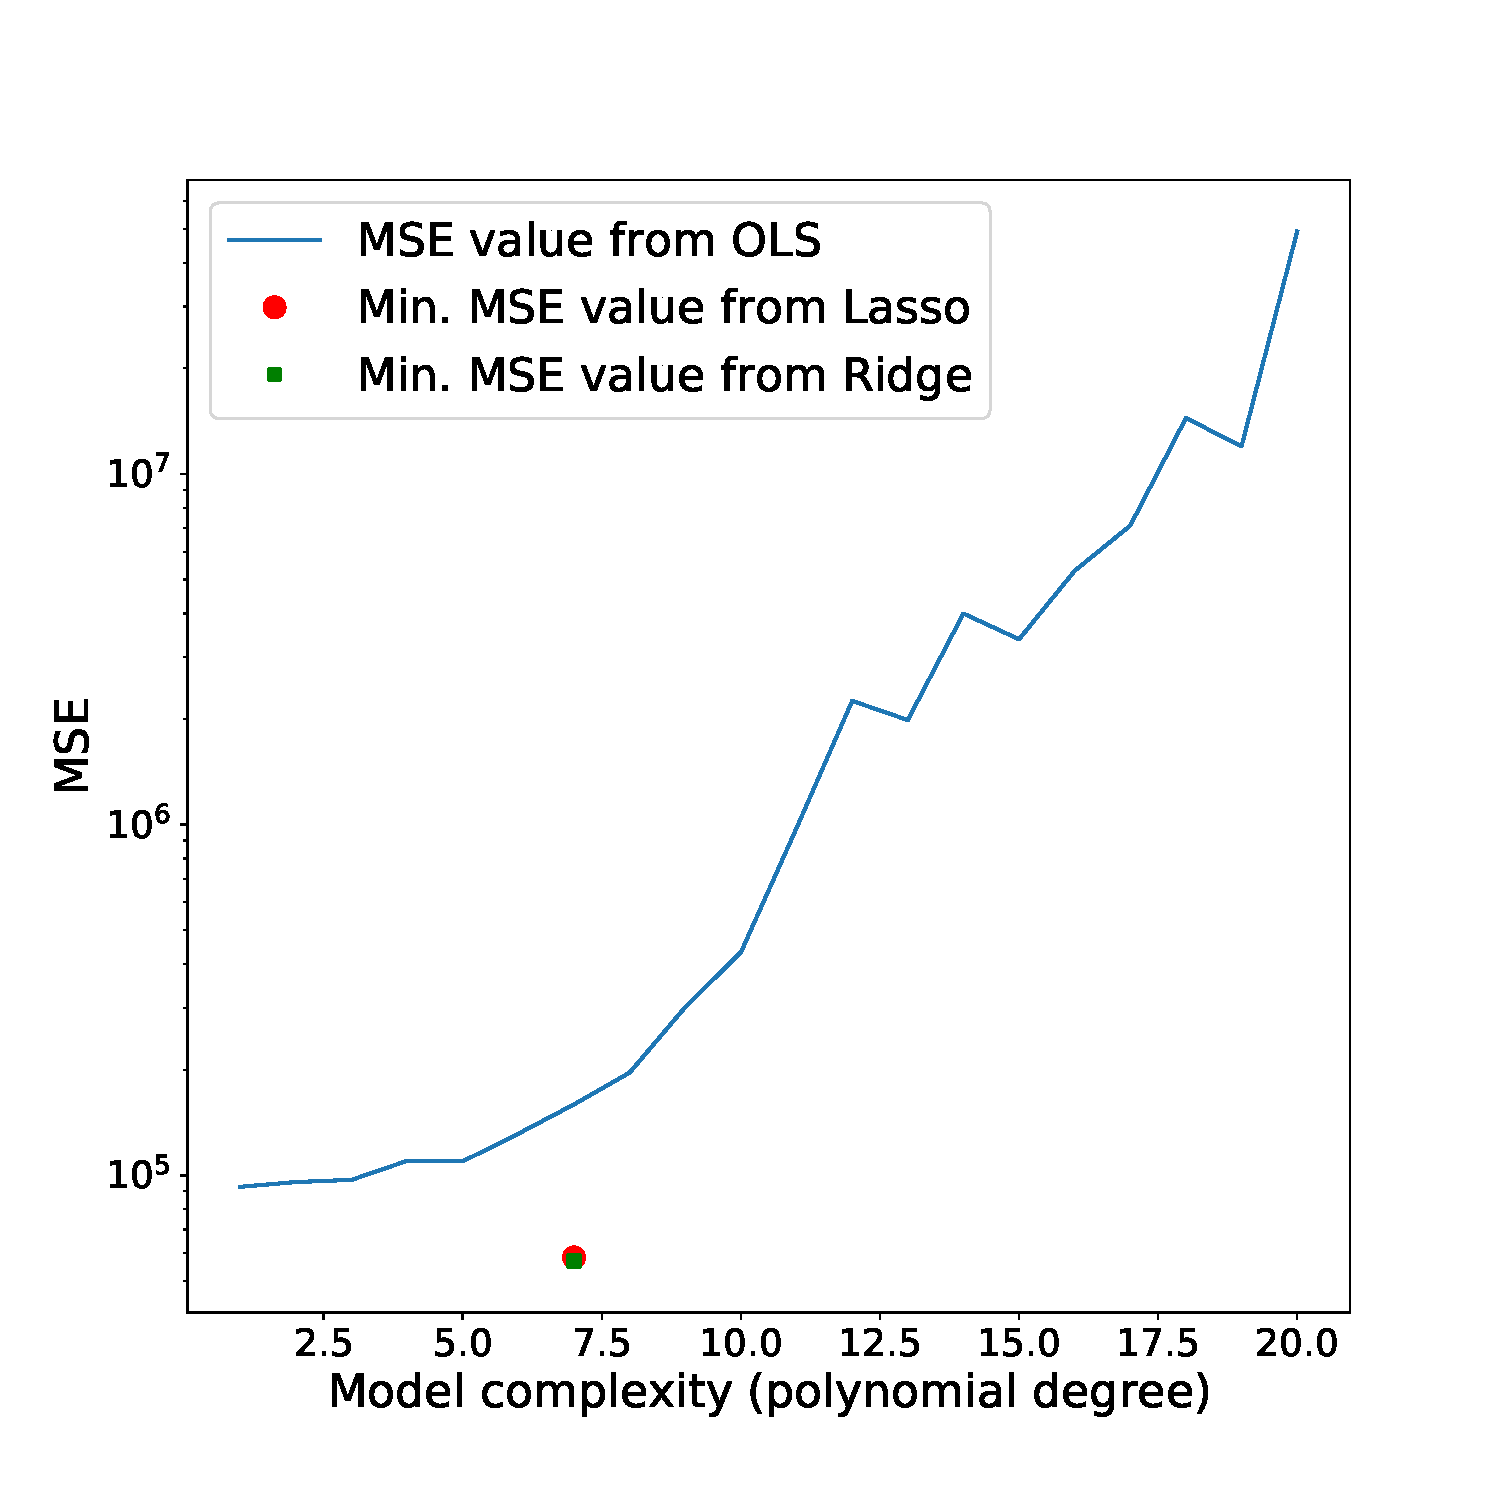
\includegraphics[width=\linewidth]{figures/optimal_mse_ols.pdf}
	\captionof{figure}{The MSE of our fit on the terrain-data with OLS regression is plotted against different values of polynomial degree. The optimal MSE values from Ridge and LASSO regression is marked with a red and green cross.}
	\label{fig:MSE_optimal_ols}
	\end{center}
}



\section{Discussion}\label{sec:discussion}

\subsection{Franke data}

For the Franke function data we noticed a trend in the OLS parameters $\boldsymbol{\beta}^{OLS}$ that the parameters in the "middle" of Figure \ref{fig:beta-confidence}, i.e. for the parameters around $\beta_6$, had a larger confidence interval. When studying the $\mathrm{R}^2$ score and MSE for the training and test data for all three methods in Table \ref{tab:task1a-values}, the OLS method performed the best. However this was merely studied for one complexity and hyperparameter, so with the optimal values for each of the methods we might have gotten better results. But nonetheless we found that especially OLS and Ridge performed very well on our Franke Function data for that complexity and $\lambda$. 

When studying the bias-variance trade-off in Figure \ref{fig:MSE_bias_var_franke}, we saw that, as expected, the bias was high for low complexity and low for high complexity, and that the variance behaved oppositely. The bias and variance also added up to the MSE value. This indicated that for low complexity we would experience underfitting, whereas for high complexity we would experience overfitting, meaning that we would need to find the perfect point in between these extremes to find the best complexity for our method. Furthermore, we can see that the more datapoints we have, the lower the MSE score gets. 
From this figure, we can also note that the bootstrap resampling gives us a higher MSE-score. There is a risk of overfitting the Franke data to the added noise, but with the resampling techniques we uncover these potential overfits as the figures shows. 


Our constructed algorithm for the $K$-fold cross validation, showed similar results as the one from \texttt{Scikit-Learn}. A study of the time performance were not done, but we can assume a well-used module as \texttt{Scikit-Learn} will perform better. We saw in Figure \ref{fig:MSE_kfold_franke} that the $K$-fold cross validation provided lower MSE and better results compared to the bootstrap resampling, and most certainly better than with no resampling methods. We studied $5$, $7$ and $10$ folds, and found that a higher number of folds provided better results, but longer computing times.

Looking at the MSE-scores of the Ridge regression, we saw that the Bootstrap resampling yielded a lower score than the $K$-fold cross validation (see Figure \ref{fig:MSE_ridge_franke}). The same tendency was seen with LASSO regression (see Figure \ref{fig:MSE_LASSO_franke}). In both cases, the Bootstrap MSE score, as a function of the hyperparameter $\lambda$, got a higher minimum MSE score than the $K$-fold cross  validation. As expected, the test MSE score is higher than the training data for both cases. Bias and variance plotted versus the hyperparameter $\lambda$ in Figures \ref{fig:biasvariance_ridge_franke} and \ref{fig:biasvariance_LASSO_franke}  showed very low values, and though we could see a crossing between bias and variance for Ridge in Figure \ref{fig:biasvariance_ridge_franke}, we could not see that in Figure \ref{fig:biasvariance_LASSO_franke} for LASSO.

\subsection{Terrain data}

In Figure \ref{fig:MSE_ols_kfold_terrain} we looked at the different number of $K$-folds with OLS regression for the terrain data. The plot is fairly similar as the equivalent plot for the Franke data in Figure \ref{fig:MSE_kfold_franke}, in showing that a higher $K$-fold number yields a lower MSE-score for higher complexity.

In Figures \ref{fig:MSE_ridge_terain_poly10}, \ref{fig:MSE_ridge_terain_poly20}, \ref{fig:MSE_LASSO_terain_poly10} and \ref{fig:MSE_LASSO_terain_poly20} we have compared the MSE-scores as a function of the $\lambda$ for two different polynomial degrees. For Ridge regression, a polynomial degree of $10$, yielded a slightly lower MSE than for a polynomial degree of $20$. For LASSO, the result was opposite. This motivated the plots in Figures \ref{fig:MSE_optimal_ridge} and \ref{fig:MSE_optimal_LASSO} where we did a bigger run, comparing different polynomial degrees to different $\lambda$-values. Here an optimal MSE-value was found for both LASSO and Ridge regression. For our input parameters, Ridge regression scored a slightly better MSE value than LASSO regression. In Figure \ref{fig:MSE_optimal_ols} we have also compared the MSE values for different complexities found with the OLS regression. The plot also contains the optimal MSE for Ridge and LASSO regression. In this plot, the Ridge and LASSO optimal values are hard to distinguish between. We can see that the OLS did not perform as well as Ridge or LASSO regression for the chosen parameters.

\section{Conclusion}\label{sec:conclusion}
Three different regression methods, OLS, Ridge and LASSO has been analysed using the bootstrap resampling method and  $K$-fold cross validation. We used the different methods on the Franke functions, with added noise, and also real terrain data. The model complexity was varied as increasing values of polynomial degrees (for OLS, Ridge and LASSO) and the hyperparameter $\lambda$ (for Ridge and LASSO). Here, the OLS regression proved to give the lowest, i.e. best, MSE score for our chosen parameters. 

For the Franke data, we saw that the resampling methods gave us a more reliable value for the MSE. For the remaining "real"-data analysis, we used the $K$-fold cross validation to resample the data.

For the terrain data, and our input parameters, we saw that the OLS regression scored a much worse MSE than LASSO and Ridge regression. The latter gave the lowest MSE score, and we thus conclude that it would be the optimal model to use for the terrain data.

\section{Outlook/remarks}\label{sec:outlooks}
For the Franke function data, we found that the OLS provided the best results, but this was for a limited analysis of $\lambda$ and complexity values of LASSO and Ridge, so with even further analysis and finding the optimal values, the results for these methods might have improved.

In the case of the terrain data we found the optimal values of $\lambda$ and complexity for Ridge and LASSO. The Ridge regression performed the best of all three methods in this case. To illustrate how well it would reproduce the terrain data it could have been used to recreate and plot the terrain data prediction. However as our analysis proved that Ridge gave the best MSE, we could still conclude that it was the best method for the terrain data. 

The repetition loops discussed in Section \ref{sec:meth}, was only done for $10-25$ repetitions, as this proved to be rather time-consuming. Ideally we could have done more repetitions.

\newpage


\appendix
\section{Appendix}
\subsection{Code}\label{sec:codeappendix}
The code developed in this work can be found at the following GitHub repository: \url{https://github.com/tellefs/ML-projects}.



\bibliography{References}

\begin{thebibliography}{999}

\bibitem{franke}
R. Franke, \textit{A critical comparison of some methods for interpolation of scattered data} (No. NPS53-79-003). NAVAL POSTGRADUATE SCHOOL MONTEREY CA. (1979).

\bibitem{morten}
Morten Hjorth-Jensen, \textit{Data Analysis and Machine Learning} - Lecture notes, fall 2020.

\bibitem{hastie}
Hastie, Trevor J., et al. \textit{The Elements of Statistical Learning: Data Mining, Inference, and Prediction}. 2nd ed., Springer Science Business Media, 2009.

\bibitem{bias-variance}
Maksym Zavershynskyi, \textit{MSE and Bias-Variance decomposition}, 2017. \href{https://towardsdatascience.com/mse-and-bias-variance-decomposition-77449dd2ff55}{https://towardsdatascience.com/mse-and-bias-variance-decomposition-77449dd2ff55}, accessed 29.09.2020.


\bibitem{terrain}
US Geological Survey, \href{https://earthexplorer.usgs.gov/}{https://earthexplorer.usgs.gov/}.


\end{thebibliography}

\end{multicols}
\end{document}
